\documentclass[harvard]{lincolncsthesis}

%TC:envir python [ignore] displaymath

% Packages you intend to use
% ..

% For example, if you want to render 
% the document in a different font you can
% use something like: 

% \usepackage{gentium}

\usepackage{url}

% Put the correct details in here
\author{Alfie Atkinson}
\studentnumber{25715017}
\email{25715017@students.lincoln.ac.uk}
\thesisDegree{MComp Computer Science}
\thesisSubmissionDate{May 2024}

% If your thesis title spans over three lines, prepend the command with \Large!
\title{\bfseries Detecting Sentiment in Online Discourse: A Machine Learning Approach for Brand Monitoring}

% Supervisor details
\thesisSupervisor{Dr. Zied Tayeb}

\thesisLogoPath{figures/logo.pdf}  

% Add in the .bib files you wish to add 
% into your document here. If you want to
% include others, just copy this line and
% change the path!

\addbibresource{bib/references.bib}


% This thesis template also supports rendering
% a ludography. To cite games, make sure your reference
% in your bib file has keywords={game} in the bibtex item.
%
% See the bib file below for an example.

\addbibresource{bib/ludography.bib}

\setlength{\parindent}{0.635cm}
\setlength{\parskip}{0pt plus 1pt}

\begin{document}

\maketitle

\begin{acknowledgements}
Firstly, I would like to thank my supervisor, Zied Tayeb, for supporting me and informing me throughout the development and documentation of this project.

I would also like to thank my family and friends, for providing me with the emotional support needed to accomplish a project larger than anything I have ever been able to previously.

Additionally, I would like to thank the people who tested the artefact and provided valuable insight necessary for the iterative development of this project.

Finally, I would like to thank all of the great minds who work tirelessly to provide the computer science community with meaningful research into the various exciting technologies within the field of machine-learning. Without their prior research, it would not be possible for me to make this accomplishment.
\end{acknowledgements}

\begin{abstract}
Here is the abstract for this project report.
\end{abstract}

\thesisTables
\thesisBodyStart

\chapter{Introduction}
% A short overview of the project and contents of the report.
\section{Project Overview}
This project aims to enable users to determine the collective sentiment surrounding a specific product or brand through the use of Natural Language Processing (NLP).

Sentiment analysis, also known as opinion mining, is the process of using NLP techniques in order to determine the sentiment or emotion expressed in a passage of text. The goal of this process is to classify a text as either positive, negative, or neutral. The key steps of this process are as follows:
\begin{itemize}
    \item Taking a text input, this could be a sentence, paragraph, or document. In the case of this project, the input will be a social media post.
    \item Before the text can be analysed, it must undergo preprocessing. This involves removing punctuation, stop words (words that don't carry much meaning, such as ``the'', ``is'', or ``and''), converting to lowercase, and possibly tokenising (splitting the text into words or tokens).
    \item To analyse the text, it is inputted into a pre-trained sentiment classification model. This model will return a prediction of the sentiment within this text and assigns a classification to it based on the patterns it has learned in training.
\end{itemize}

This project will be testing and harnessing various machine learning models to analyse the sentiment of posts on social media. These posts will be scraped from the internet using various Application Programming Interfaces (APIs), and the process will be made accessible for a layperson via an application with a user friendly interface.

% A section providing wider context surrounding the project and why it is important.
\section{Context}
With the rise in use of the internet as both a place for discussion and a news source, it is becoming increasingly important for companies to monitor and understand what is being said about their brand online.

The swift expansion of the internet and social media has lead to customers abandoning company sites in favour of other networks for the purpose of sharing their opinions of a brand. This is an issue for brand monitoring, as it can be difficult to identify and understand problems that users may have with a product before it has been spread to millions of people.

In general, it now seems more effective to collect and analyse data from social media rather than investing in other means. This projects significance cannot be understated for the purpose of brand monitoring.

% A section detailing the motivations for the project by outlining the issues it solves.
\section{Motivations}
Traditional methods of gathering public opinions are through the use of surveys and focus groups. These methods can be tedious and expensive to set up, as well as not really being as effective as may be necessary.

Surveys involve preset questions which can be interpreted differently to how the surveyor intended, it is also hard to detect emotions without the survey being in the form of an in-person interview, which is a slow process and more expensive to conduct. 

Focus groups can be susceptible to `groupthink' and dishonest responses as a by-product of the group setting. There is also the possibility of the results of the focus group being skewed towards one member who is louder than the rest, and even the focus group as a whole could skew results by not accurately representing the target audience.

On top of this, even existing sentiment analysis approaches have their limitations, many are not accessible to the average user as they have complicated or no Graphical User Interface (GUI). They also do not monitor sentiment in real-time, and do not have a high level of user customisation. I also want to be sure to mitigate any ethical issues related to data privacy and bias by ensuring that my data is abstracted upon collection, and bias from things such as bot accounts is prevented.

There are several other issues with these approaches and they will be addressed in depth later in the report, where it will provide the advantages of using machine learning for sentiment analysis and how it tackles the issues with traditional methods.

% A section to outline the main objectives of the project.
\section{Objectives}
The aim of this project is to create a piece of software that is easy to set up and use, which will provide live insights into online sentiment pertaining to a specific brand. It has several distinct objectives which must be met for it to be considered a success.

Firstly, the program will implement one or more machine learning models for the use of sentiment analysis. It will allow the user to change between different models, and also provide their own training data rather than using the pre-trained models. I will aim to have at least 85\% accuracy with the models, however this will be subject to the quality of the training data.

Secondly, the program will provide a way for the user to input their brand or product name. It will then use the X (formerly known as Twitter) API to collect thousands of tweets about the product, abstract them into just text, and then predict their sentiment with the trained models. I also wish to allow the user to provide their own collected text passages about their product.

Finally, an accessible GUI must be created which allows the user to easily access all the capabilities and features of the program. This GUI will give the user the ability to search their brand or product name, review the results of the search, and save the results of the search. The user will also be able to change various settings, such as the model and training data used. This aims to create a user friendly environment so that the programme is easy to use.

Achieving these objectives is critical to the success of this project, as they all contribute to the effectiveness and efficiency of the programme.

% A section detailing the structure of the report following the introduction.
\section{Report Structure}
The next chapter of this report is a critical evaluation and review of academic literature that is relevant to this project. It will provide a strong foundation for my work and will establish clear links between existing research and the objectives of my project.

Following this, the third chapter of my report will present a further analysis of the specific requirements that my solution must satisfy in order to achieve the desired results. This will encompass both the functional and non-functional requirements of the solution, as well as a risk analysis and the testing/evaluation methodologies for the artefact.

Chapter 4 will outline the design and methodology implemented in this project. It will discuss the project management approaches and the software development methodologies used. It will also discuss algorithm and model choices, design considerations, analysis methods, performance evaluation strategies, and other relevant aspects of the project design and execution.

Chapter 5 will provide a clear, detailed description of every component which contributes to the software's implementation, documenting important sections of code where relevant. Here It will also show the results of any testing and evaluation results that are gathered during the development of the artefact.

Chapter 6 will then present the results of the implementation. Here I will reflect on the project and discuss how it meets the original objectives that were set out to be achieved, and the project's significance within the world of brand monitoring.

Finally, the project will be summarised within a conclusion, highlight its achievements, limitation, and implications. It will reflect on the accomplishments of this project and address any unresolved issues.

\textit{Note: this report is a total of 11,793 words long. Throughout this report there will be references to work from the previous project proposal \citep{atkinson2023proposal}, and the interim report \citep{atkinson2024interim}.}

\chapter{Literature Review}
\section{Introduction to Sentiment Analysis and NLP}
Sentiment analysis is a key area of Natural Language Processing (NLP). It is used to extract and analyse the opinions and emotions from written passages \citep{dhuria2015sentiment, mishra2022data}. This technique is useful in social media and e-commerce sites \citep{anny2022sentiment}, as there is an abundance of data with over 500 million daily posts on X (formerly known as Twitter) alone \citep{sayce2022twitter}.

\section{Instances of Public Sentiment Impacting Brands}
Historically, public sentiment has a significant impact on a brand's credibility, as evidenced by a range of studies. \citet{berestova2022consumers} found that consumers prefer to engage with brands which take public stances on real-world issues. \citet{mostafa2013more} further supports this, writing about the generally positive sentiment surrounding various large brands on social media.

In 2016 Samsung released the Samsung Galaxy Note 7 Smartphone. Shortly after its release there were cases of the phone overheating and sometimes `exploding. This caused massive backlash online, with many users of X posting negatively about the incident \citep{kang2019social}.

\citet{lange2011people} emphasizes the importance of sentiment analysis for managing reputational risk, especially in response to incidents like the Galaxy Note 7. \citet{hu2017analyzing} also highlights the part social media users play in shaping a brand's perception, user loyalty, and advocacy.

These studies all show the crucial role that public sentiment plays in shaping a brand's reputation and success.

\section{Nuanced Issues in Sentiment Analysis}
While catastrophic events such as the Galaxy Note 7 incident may capture immediate attention, the use of sentiment analysis to identify more subtle issues has been the interest of a range of studies. \citet{pang2004sentimental} proposed a machine-learning method which focused on the subjective parts of a given text, that may identify specific complaints or criticisms. \citet{zhou2016linguistic} highlighted the distinct properties of complaints and praises, while \citet{nasukawa2003sentiment} emphasized the need to identify semantic relationships between expressions and the subject matter.

However, \citet{d2019sentiment} gave a new perspective on sentiment analysis by discussing it's limitations and proposing a dual sentiment analysis approach. This approach would create sentiment-reversed reviews, meaning that for each training and test review, a corresponding reversed review would be generated. This technique aims to capture the dual nature of a given sentiment by considering both positive and negative perspectives. A technique such as this can be particularly useful for social media posts, as there is a strong likelihood that the posts contain both positive and negative sentiment.

\section{Explosive Growth of Social Media Data}
The surge in social media usage, as highlighted by \citet{dean2023social}, underscores the increasing need for efficient data analysis techniques for market research, where social media data can provide valuable insight \citep{camacho2021new, ausat2023utilisation}.

To meet this need, \citet{malic2019social} emphasizes the importance of systematic data collection, secure storage technology, and efficient querying of said data. This can be done through the parallelisation of data extraction using various web scraping tools and APIs.

\section{Goals and Challenges of Market Research}
Market research plays a crucial role in providing information for management decision-making, with the primary goals being to analyse market conditions, determine consumer segments, and assess sales possibilities \citep{cvijanovic2014market}. However, the increasing volume and complexity of data, changes in consumer preferences, and growing competitive pressure present significant challenges with traditional techniques \citep{shikovets2023digital}. Traditional data collection methods such as surveys and focus groups are also limited in their ability to accurately capture sentiment due to issues with polarity shift, data sparsity, and binary classification \citep{abirami2017survey}. 

To address these challenges, the industry is undergoing significant changes, including the integration of digital tools, the use of advanced technology, and the adoption of new research techniques \citep{barbu2013eight}. \citet{vikram2020use} talk about how brands are increasingly relying on user feedback to improve their products and services. This feedback can take various forms, such as social media posts and product reviews \citep{kanev2023leveraging}. \citet{kupec2015marketing} talks about how clients are increasingly seeking innovative approaches that provide higher value information, and \citet{gerdes2008integrative} highlights how valuable the integration of both qualitative and quantitative feedback is, providing a more comprehensive understanding of consumer sentiment.

Overall, brands are interested in feedback that can help them enhance product quality, service quality, and design, and that can provide insights into user experiences and perceptions efficiently and effectively.

\section{Machine-Learning Models}
Both traditional machine-learning models and deep-learning models can be used in sentiment analysis. Traditional models such as logistic regression and decision trees, while robust and allowing for rapid prototyping, may not perform as well as deep-learning models when it comes to large datasets \citep{rajnayak2017traditional}.

In fact, \citet{kansara2020comparison} and \citet{kamruzzaman2021comparative} revealed the superiority of deep-learning models over traditional machine-learning models. Both found that deep-learning models often outperformed traditional models in accuracy and performance.

To further support this, \citet{dhola2021comparative} demonstrated the effectiveness of various deep-learning models such as Bidirectional Encoder Representations from Transformers (BERT) and Long Short-Term Memory (LSTM). \citet{kamruzzaman2021comparative} also highlighted the success of models like Single Convolutional Neural Network (CNN) + FastText and 2-L CNN + Gated Recurrent Unit (GRU) in sentiment classification specifically.

While BERT has been widely acclaimed for its performance in NLP tasks, its superiority over LSTM is not universal. \citet{ezen2020comparison} found that for intent classification with small datasets, LSTM outperformed BERT. However, \citet{rangila2022sentiment} reported that BERT achieved higher accuracy and efficiency in sentiment analysis tasks. Demonstrations show that BERT is very effective in lexical simplification \citep{qiang2021lsbert}, which may be useful for analysing social media posts.

Linking back to \citet{d2019sentiment}, \citet{yin2023prompt} talk about their progress using BERT for Aspect-Based Sentiment Analysis (ABSA). This technique aims to predict sentiment polarity to specific aspects within the given sentence, allowing for more nuanced feedback to be detected. \citet{yin2023prompt} proposed a Prompt-oriented Fine-tuning Dual BERT (PFDualBERT) model which can capture complex semantic relevance and consider scarce data samples simultaneously.

\section{Data Collection Through Web Scraping}
Web-scraping is a data collection technique for automatically capturing data surrounding certain topics, which is used more frequently than ever in social research \citep{marres2013scraping}.

\citet{hernandez2018web} presented a methodology for collecting historical tweets by using web-scraping, and \citet{baskaran2018automated} proposed a way to extract structured data records from health discussion forums using semantic analysis. On top of this, \citet{dewi2019social} developed a system to scrape social media websites such as Facebook and X using their respective APIs, along with regular expressions to suppress overload information, presenting relevant information.

\section{Ethical Considerations}
Systems for Automatic Emotion Recognition (AER) and sentiment analysis can facilitate amazing progress (e.g., improving public health and commerce), however it can also be used maliciously (e.g., suppressing dissidents and manipulating voters) \citep{mohammad2022ethics}. \citet{veeraselvi2014semantic} and \citet{basiri2014exploiting} both emphasize the importance of considering context and history of user comments, as well as the potential bias in the data. \citet{liu2010sentiment} and \citet{chandra2015sentiment} further highlight the need for transparency and accountability when using sentiment analysis tools, particularly in the face of challenges such as manipulation, privacy concerns, and economic impact.

\citet{krotov2020tutorial} provide a specific list of questions that a researcher must consider when web scraping, such as Terms of Service (ToS) compliance, data protection, and privacy policies. \citet{fiesler2020no} and \citet{mancosu2020you} both talk about the ambiguity and inconsistency that is present in the ToS for social media platforms, which can make it difficult to be certain that rules are followed. Whereas \citet{zia2020there} focuses more on the fact that harvesting online data could infringe on a user's privacy, emphasizing the importance of anonymity when storing data.

\citet{steinmann2016theoretical} propose a theoretical framework for ethical reflection in big data research, providing a privacy matrix that intersects ethical concerns with different contexts of data use. This approach offers a practical way to assess the ethical implications of data collection and use.

\section{Challenges and Mitigation Strategies}
There are many challenges in data analysis, and those challenges are multifaceted. It is difficult to be sure to extract only relevant, valuable information from large datasets, all while abiding by legal and ethical obligations and responsibly using the findings of data analysis \citep{nayak2002intelligent, choenni2021using}.

Due to the significant amount of data that can be contained within these datasets, there are also various resource and scalability issues that may arise \citep{duffield2014challenges}. The possibility of failure in data analysis makes the importance of mitigating these challenges very apparent \citep{staegemann2020determining}.

To address these problems, data sampling strategies, responsible usage of analyses, and planning for and understanding potential failures are imperative.

\chapter{Requirements Analysis}
\section{Target Audience Identification}
The main target audience for this application consists of marketing professionals, product managers, and business owners in various industries. The main industries being the technology, retail, and hospitality sectors. However, it should be made available and accessible to other industries and audiences, including public users.

A study by \citet{marketing2023survey} found that 74.6\% of people working in marketing are between the ages of 26 and 45, meaning that they tend to be within the `millennial' age group, a group which seems to be more in touch with technology and social media than older generations \citep{pew2019millennials}. However, a study by \citet{harvard2018research} found that the top 0.1\% of startup companies based on growth in the first 5 years have founders aged 45 on average, only getting older as the company progresses. This means that the programme must be accessible to a broad age range, even those who may be unfamiliar with technology.

In conclusion, while there are some demographics that this application should cater towards, it should also be made with all demographics of people in mind.

\section{Functional Requirements}

    \subsection{Data Collection and Preprocessing}
    The programme should be able to collect data from various social media platforms, such as X and Reddit. It should also be able to accept JSON files containing reviews for the brand. The data should be effectively stripped of any personal data, and made completely anonymous before being stored. The programme should also remove noise within the text such as punctuation, stop words, and special characters. Finally, text normalisation techniques such as tokenisation, stemming, and lemmatisation should be applied to ensure consistency in the data.

    The aim is to have the programme remove 100\% of any personal data and noise that may be present within the social media posts or reviews. It is imperative that this goal is met in order for the application to be effective ethically sound.

    Both X and Reddit have well documented APIs which will be used to scrape posts relevant to the search term. There are python libraries which make it possible to access these APIs, and also libraries which allow for the reading of JSON files.

    It should be ensured that the collected data is definitely related to the specified search term in order to provide meaningful insights.

    This requirement should be met within the first week of development.

    \subsection{Sentiment Analysis}
    The programme will implement BERT for sentiment analysis and the proposed PFDualBERT for capturing complex semantic relevances and consider scarce data samples simultaneously. It will be able to predict whether the general sentiment around a given search term is positive, neutral, or negative; it will be able to predict sentiment polarity about specific aspects within the texts.

    The predictions should have a sentiment classification accuracy greater than 85\%, to ensure that it is overall robust and effective for analysing public sentiment.

    State-of-the-art sentiment analysis such as LSTM, BERT and the proposed PFDualBERT will be explored.

    The sentiment analysis results should provide valuable insights for brand monitoring and decision-making.

    This requirement should be met within the first three weeks of development.

    \subsection{Real-Time Analysis}
    The programme will be able to analyse social-media data in real-time; the user will be able to set how often they would like sentiment to be re-evaluated, and the data will be updated accordingly.

    The programme should be able to find all new social-media posts since the last update with no more than 1 minute delay, ensuring swift and consistent real-time results.

    Data that has already undergone analysis will be saved to be recalled upon when the user wishes to view the data, this means that the programme only needs to analyse new posts every interval.

    The user will be provided with timely insights into the evolving sentiment surrounding their brand/product.

    This requirement should be met within the first four weeks of development.

    \subsection{Graphical User Interface}
    The application will have a user-friendly interface which allows the user to interact with the system, change settings, and view various graphs containing the sentiment analysis data over chosen time periods.

    A minimum usability score of 8 out of 10 should be achieved in user testing surveys conducted with targeted users.

    Modern GUI design principles will be implemented, alongside iterative usability testing with target users.

    Ensuring that the user interface effectively facilitates any user interactions is imperative for it to be a desired tool. Data being represented correctly within an interface is necessary for the results to be useful to the end-user.

    This requirement should be met within the first eight weeks of development

\section{Non-Functional Requirements}

    \subsection{Performance}
    System performance will be optimised to handle a minimum of 10,000 social media posts per hour, ensuring that a large amount of data can be captured.

    It should be able to achieve an average response time of less than 360 milliseconds for data retrieval and sentiment analysis processing.

    Algorithms will be optimised to take as little time as possible while still performing tasks correctly.

    This assures that the programme can meet the demands of processing large volumes of social media data in real-time.

    This requirement should be met within the first four weeks of development.

    \subsection{Usability}
    User testing sessions will be conducted with target users in order to evaluate the usability of the system interface.

    A minimum usability score of 8 out of 10 should be achieved in user testing surveys conducted with targeted users.

    Feedback will be gathered from users through usability tests and this feedback will be iterated on until the desired score is achieved.

    This will ensure that the application GUI is intuitive and easy to navigate for users of varying levels of technical experience.

    This requirement should be met within the first ten weeks of development.

    \subsection{Security}
    A secure login mechanism will be implemented to control access to the system and protect stored data. All saved data will be encrypted.

    Encryption methods such as Advanced Encryption Standard (AES) encryption will be employed within the programme along with a secure login system that makes data inaccessible without the correct password.

    The programme will use cryptography for AES encryption to implement secure login and data encryption features.

    By making sure the programme and data are secure, users can be sure that data is kept confidential and secure.

    This requirement should be met within the first six weeks of development.

    \subsection{Reliability}
    The application will function reliably without crashes or unexpected errors, providing consistent performance under all usage scenarios.

    Error handling and logging mechanisms will be used to track and address any issues that may be raised during the application's execution. The performance and uptime of the application will be monitored to achieve at least a 99.5\% reliability rate.

    Python's built-in exception handling will be used, and logging modules will capture errors. Testing frameworks such as pytest will be used to validate the application's reliability.

    User trust and satisfaction will be maintained by ensuring the programme operates reliably, minimising downtime and preventing data loss or corruption.

    This requirement should be met within the first eight weeks of development.

    \subsection{Accuracy}
    The programme should accurately categorise sentiment in text data, providing the user with reliable sentiment scores and classification.

    Data validation checks will be used to ensure the accuracy of the sentiment analysis is at least 85\%.

    Well-established sentiment analysis libraries will be used, such as BERT. Unit tests and validation checks will be used to ensure that the desired accuracy is achieved.

    This will allow users to trust the programme and its analysis of social media data surrounding the search term.

    This requirement should be met within the first four weeks of development.

\section{Risk Analysis}

    \subsection{Data Security}
    There is risk of data leaks or unauthorised access to sensitive information. This can be overcome by implementing robust encryption techniques such as AES encryption and secure storage to protect data. All data will be encrypted before ever being stored, and it will require a password to decrypt for viewing.

    \subsection{Performance Issues}
    It is possible that the application may crash or have slow response times during sentiment analysis. To overcome this, code should be optimised, error handling should be implemented, and performance testing should be conducted to ensure that the application operates efficiently under all conditions.

    \subsection{Algorithm Accuracy}
    There is the possibility that the sentiment analysis results may lead to incorrect insights by not being accurate enough. This is easily mitigated by validating the sentiment analysis algorithms using a diverse dataset, and refining algorithms based on these test results until an accuracy above 85\% is achieved. 

    \subsection{Poor User Experience}
    The GUI could have poor usability or be seen as unintuitive, which would affect user adoption. To mitigate against this, user testing will be conducted to gather feedback on the GUI design. This feedback will then be iteratively acted upon until user satisfaction is high enough.

    \subsection{Terms of Service Changes}
    Social media platforms frequently update their ToS, which could impact the programme's ability to effectively scrape for social media posts or access the API. This can be countered by regularly monitoring the chosen social media's ToS and by implementing flexibility in the programme's design to be able to adapt to API changes.

    \subsection{Ethical Regulation Changes}
    There is always the possibility that changes with ethical regulations may impact the ways sentiment analysis can be used. In order to prevent this being a problem, it is important to stay informed about relevant regulations and ethical guidelines. It is also important to be sure to reflect on the ethics of the project at all stages.


\section{Requirements Validation}
Ensuring the robustness and reliability of the tool necessitates rigorous validation of both functional and non-functional requirements. To validate the functional requirements, the application will undergo a series of unit tests, integration tests, and system tests to be sure that each feature operates as intended and meets the specified criteria. For example, the login system will be tested to verify its functionality in securely authenticating users, while data encryption will undergo tests to confirm the safeguarding of sensitive information.

Non-functional requirements will be validated through comprehensive testing and performance monitoring. Security measures, including data encryption, will be rigorously evaluated to ensure compliance with industry standards and best practices. Moreover, the reliability and accuracy of the sentiment analysis algorithms will be assessed by comparing the tool's predicitions against manually annotated data sets to measure accuracy and consistency.

On top of this, User Acceptance Testing (UAT) will be conducted to validate that the application meets the expectations and needs of the target audience. This involves soliciting feedback from intended users of the programme to gauge the tool's usability, effectiveness, and overall satisfaction.

\chapter{Design \& Methodology}
This section aims to outline the basic design and architecture of the artefact.

\section{System Architecture}
The sentiment analysis tool will be built as a desktop application developed in Python. The system architecture consists of three main elements: the GUI, the chosen machine learning model for sentiment analysis, and the integration with social media APIs for data retrieval. This section will go into more detail on the specific design and architecture of the application.

\begin{figure}[h]
    \centering
    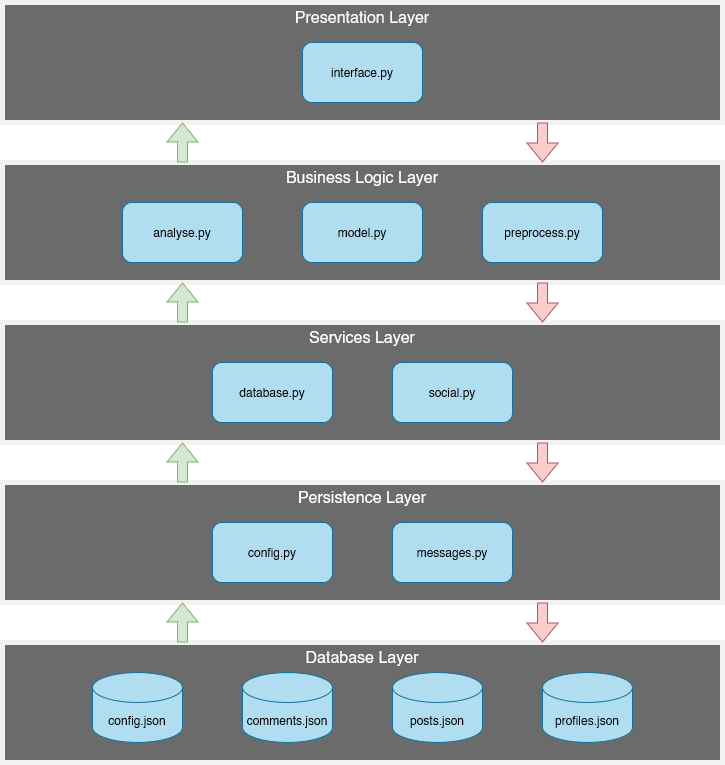
\includegraphics[width=0.8\textwidth]{figures/system-architecture-layers.png}
    \caption{Proposed system layer architecture.}
\end{figure}

    \subsection{Architectural Style}
    The system uses a layered architecture, dividing the application into distinct layers containing components based on their function and responsibility. This style promotes modularity, scalability, and maintainability by separating concerns and enforcing clear boundaries between different parts of the system. The layered architecture also allows for easy integration of new features int he future.

    \subsection{Layers and Components}
    The system comprises of five main layers: presentation layer, business logic layer, services layer, persistence layer, and database layer.

        \subsubsection{Presentation Layer}
        The presentation layer is responsible for presenting the processed and analysed data to the user. In \pinline{interface.py} there will be various classes for building and handling the windows and their layouts; there will also be classes for handling functions on other threads in order to preserve the functionality of the GUI while long running operations are in progress.

        \subsubsection{Business Logic Layer}
        The business logic layer is responsible for interpreting the data provided by the layers below. \pinline{analyse.py} will handle the analysis of data, for example the creation of a line chart which plots the sentiment over a given time frame. \pinline{model.py} will contain a class for the machine learning model which will handle training of the model as well as making predictions using the model. Finally, \pinline{preprocess.py} will be responsible for processing and cleaning text before training/making predictions.

        \subsubsection{Services Layer}
        The services layer is responsible for interacting with the social media APIs and the data sources. In this layer there is \pinline{database.py}, which collects and manipulates post data from the APIs and any stored, previously collected data. Meanwhile, \pinline{social.py} will contain classes for the social media APIs, with functionality for scraping posts with given search terms.

        \subsubsection{Persistence Layer}
        The persistence layer is responsible for the persistence of configuration, settings, and logging errors and messages. It will consist of two modules: \pinline{config.py} and \pinline{messages.py}, which will have simple functions intended for retrieving data from the database layer and sending messages to the console respectively.

        \subsubsection{Database Layer}
        The database layer is responsible for storing persistent data used by the application. \pinline{config.json} will store all of the configuration settings of the app, while \pinline{profiles.json} will store the specific configurations for each profile in terms of searching social media. Lastly, \pinline{posts.json} and \pinline{comments.json} will store collected posts and comments respectively, with all the necessary information for analysis such as the body text, the amount of favourites, the predicted sentiment, and specific to comments, the parent post (to allow for contextual analysis).

    \subsection{Key Components}
    The key components and their important classes are as follows:
    \begin{itemize}
        \item \pinline{interface.py}: this module will handle everything to do with the GUI.
        \begin{itemize}
            \item \pinline{MainWindow()}: this class will be responsible for building the main window and handling any interactions the user may have with it.
            \item \pinline{SubWindow()}: there will be various classes for handling sub-windows such as profile editor and settings.
            \item \pinline{Worker()}: this will be a class for handling multithreaded long-running tasks to keep the GUI responsive in the meantime.
        \end{itemize}
        \item \pinline{model.py}: the module for handling everything to do with the machine learning models.
        \begin{itemize}
            \item \pinline{BERTModel()}: this class will handle the training and predicting for a BERT model.
            \item \pinline{LSTMModel()}: the class for handling the training and predicting for a LSTM model
            \item \pinline{PFDualBERTModel()}: this class will handle training and predicting for a PFDualBERT model. 
        \end{itemize}
        \item \pinline{database.py}: this module will handle everything to do with the collection of data from the databases, as well as the merging of this data with new social media posts.
        \begin{itemize}
            \item \pinline{PostCollector()}: a class to collect and merge data from social media with existing stored data.
        \end{itemize}
        \item \pinline{social.py}: the module responsible for scraping social media's posts with given search parameters.
        \begin{itemize}
            \item \pinline{XScraper()}: this class will interface with the X API to collect posts for a given search term.
            \item \pinline{RedditScraper()}: this class will interface with the Reddit API to collect posts from given subreddits with given search parameters.
        \end{itemize}
    \end{itemize}

\section{Data Model}
As the artefact will involve the storage and retrieval of data, it is appropriate to model the relationships between different entities within the data. The data model consists of three entities: profile, post, and comment; each profile will have a number of posts collected for its specified subreddits, and each post will have a number of comments collected with it if this setting is enabled. Both the posts and comments databases will be in a directory labeled with the profile ID.

For this project, it was decided that json format would be acceptable for storing data, this is due to the portable, efficient, and scalable nature of json, along with the lack of a need for anything with more complex functionality. The json data will be read and temporarily stored in a \pinline{pandas.DataFrame} structure while being used by the program.

\begin{figure}[h]
    \centering
    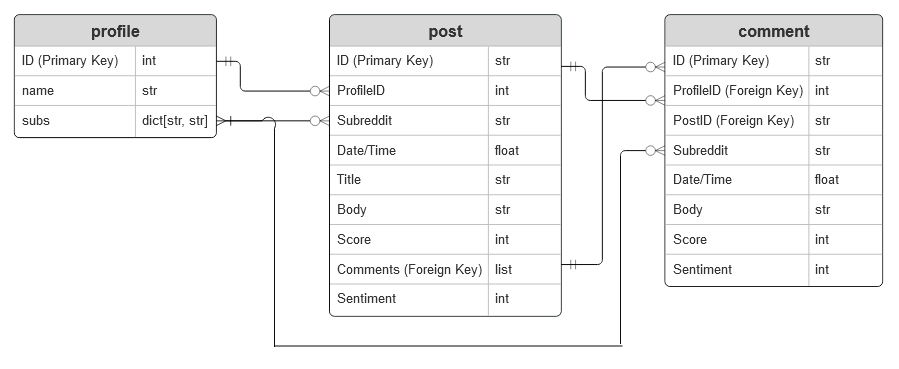
\includegraphics[width=\textwidth]{figures/database-relationship-diagram.png}
    \caption{Relational diagram showing the database structure.}
\end{figure}

\section{Graphical User Interface}
The goal of this interface is to be easily accessible, clearly show the analysis of data, and look visually professional. The interface will consist of three main windows: the main window, where majority of the functionality happens and all the data is displayed, the profile editor window, where the user can add and edit brand profiles, and finally the settings window, where the user can change settings that affect the system functionality and visuals.

The main window will consist of three main areas: the main toolbar at the top of the window containing various buttons, the time-frame selector along with text describing the profile sentiment, and an analysis panel with tabs to visualise the data in various ways.

\begin{figure}[h]
    \centering
    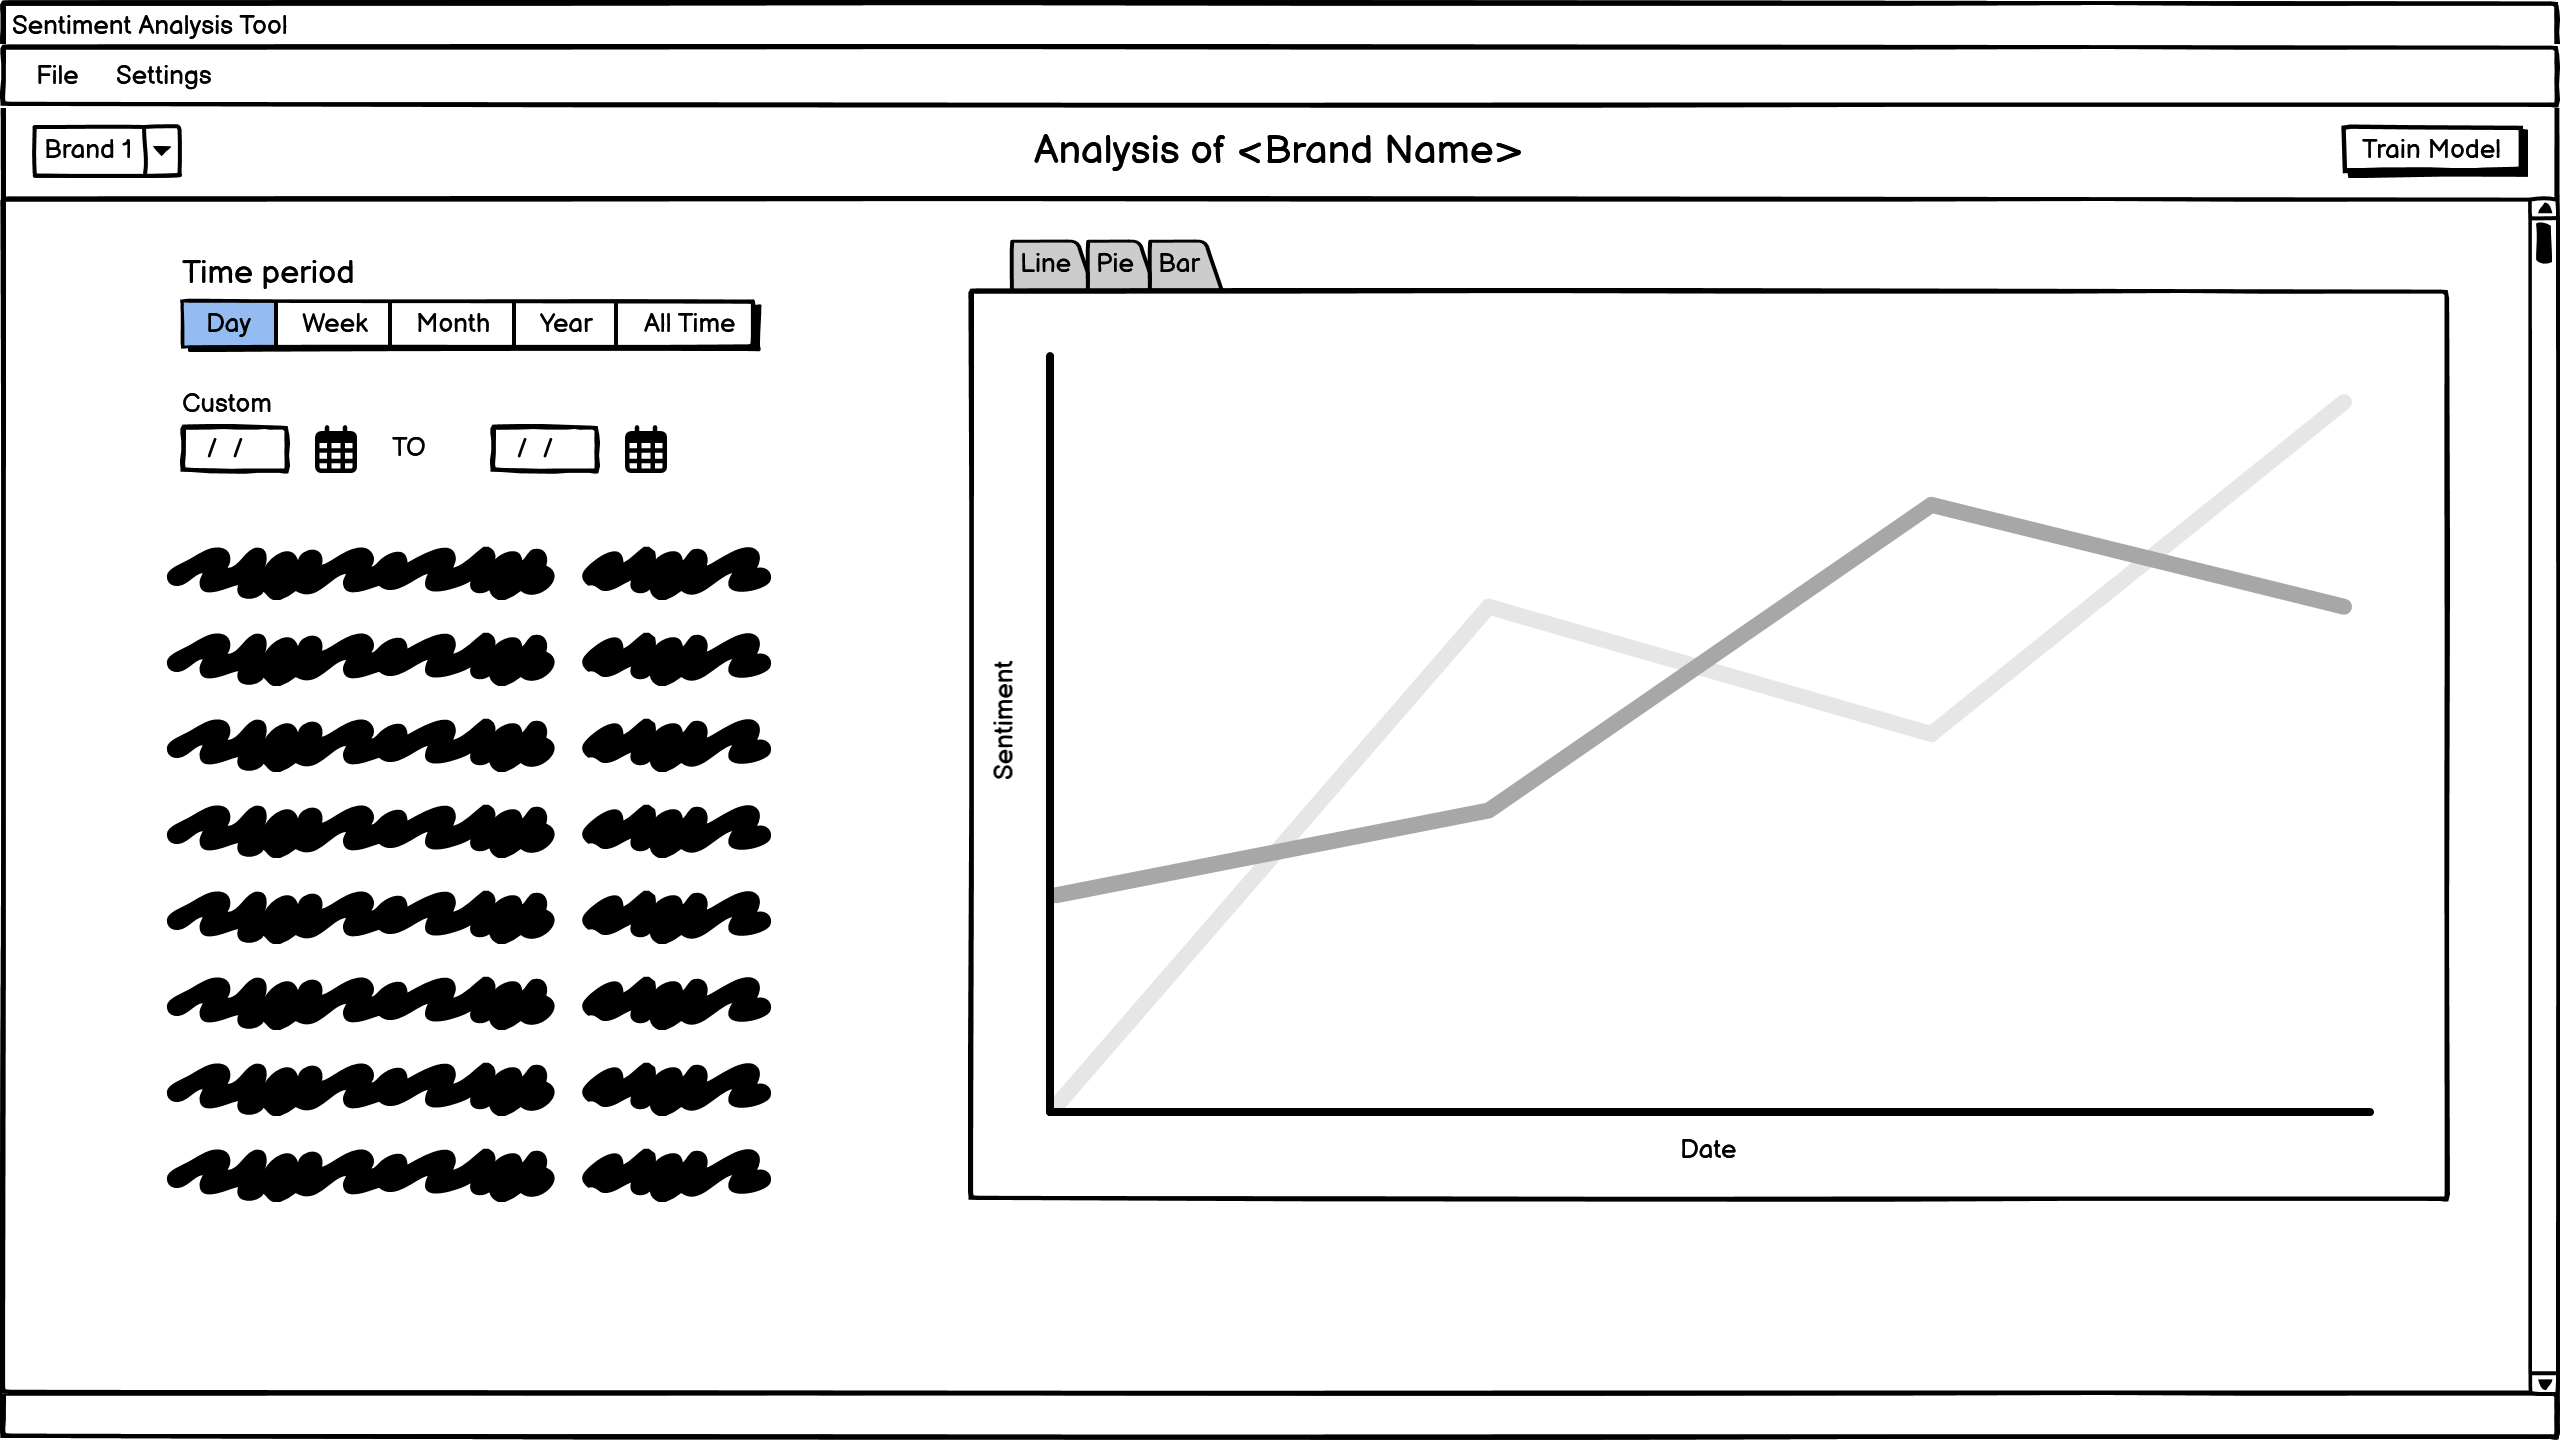
\includegraphics[width=\textwidth]{figures/wireframe-main.png}
    \caption{Wire-frame of the proposed main GUI.}
\end{figure}

The profile editor window must allow the user to easily create and edit profiles, to do this it will have a text bar for choosing the profile name, along with two buttons ``enter'' and ``delete'', which will either save or delete the profile respectively. It must also allow them to add subreddits with search terms to this profile, to do this there will be two text boxes, one for the subreddit name, and one for the terms to search for in that subreddit. When a subreddit is added to the profile, it will appear in a row below these text boxes, here the user can click the ``remove'' button to remove a subreddit and its search terms from the profile.

\begin{figure}[h]
    \centering
    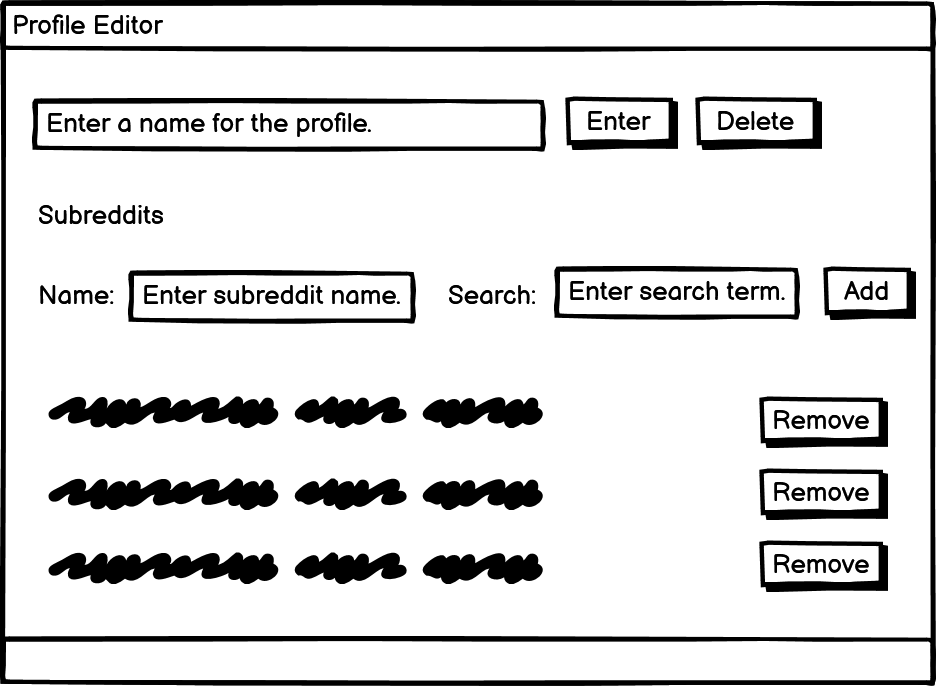
\includegraphics[width=0.5\textwidth]{figures/wireframe-profile-editor.png}
    \caption{Wire-frame of the proposed profile editor GUI.}
\end{figure}

Finally, the settings window should be easily navigable and contain various settings for functionality and visuals of the application. The different types of settings will be separated into tabs, and each setting will have its own row in the tab it belongs to.

\begin{figure}[h]
    \centering
    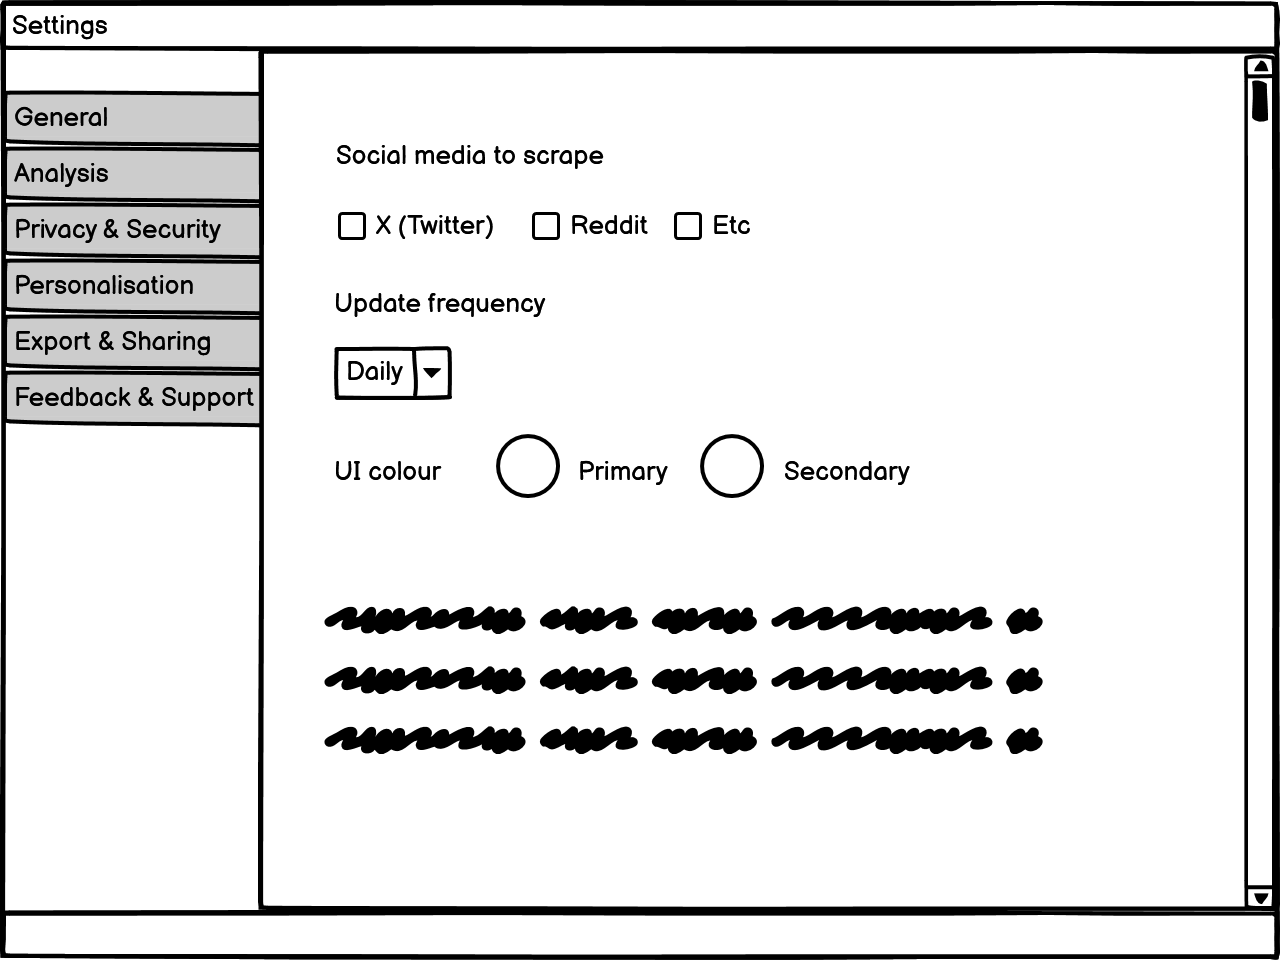
\includegraphics[width=0.7\textwidth]{figures/wireframe-settings.png}
    \caption{Wire-frame of the proposed settings GUI.}
\end{figure}

\section{Model Selection}
When selecting the model to use for this project, it was important to consider model performance, versatility, and the ability to handle complex linguistic patterns. While alternative models such as LSTM, Single CNN with FastText, and 2-L CNN with GRU have shown to be effective with NLP tasks, BERT was chosen as the preferred choice for several reasons.

    \subsection{Contextual Understanding}
    BERT's bidirectional architecture allows it to capture context information from preceding and succeeding words within the text, this addresses the complexities of language and sentiment expression highlighted by \citet{nasukawa2003sentiment, d2019sentiment}. Unlike LSTM, which processes text sequentially, BERT's bidirectional, contextual approach allows it to capture nuances and ambiguities in sentiment, making it perfect for the long-form posts prevalent in this task.

    \subsection{Pre-trained Language Representation}
    BERT is able to generalise well across diverse sentiment analysis tasks due to its pre-trained representation offering rich understanding of language semantics \citep{dhola2021comparative, rangila2022sentiment}. It's pre-trained knowledge reduces the need for extensive fine-tuning, facilitating transfer learning and aligning with \citet{malic2019social}'s recommendation of systematic data collection and storage.

    \subsection{Transformers Architecture}
    The transformer architecture allows for parallel processing and hence efficient training on large-scale datasets \citep{kansara2020comparison}. BERT's architecture and self-attention mechanism lets BERT capture long-range dependencies in long-form text, which overcomes issues with data sparsity and polarity shift often seen with traditional models \citep{abirami2017survey, kamruzzaman2021comparative}.

    \subsection{Transfer Learning}
    Due to its transfer learning capabilities, BERT is adaptable to diverse sentiment tasks with minimal labelled data, which aligns with the need in market research for innovative approaches that provide high value information \citep{vikram2020use, gerdes2008integrative}. By fine-tuning BERT on task-specific datasets, its pre-trained knowledge can be harnessed to achieve high performance in sentiment analysis.

    \subsection{Polysemy and Ambiguity Handling}
    BERT's bidirectional context modeling allows it to disambiguate polysemous words and resolve ambiguities based on surrounding context \citep{zhou2016linguistic}. This is particularly useful for analysing social media posts, where sentiment can vary based on the broader discourse and user engagement such as favourites and comments \citep{mostafa2013more, lange2011people}.

\section{Development Methodology}
For the development of this tool, an Agile-inspired approach will be used and adapted to a single-person development team. This will allow for iterative development, allowing for flexibility and adaptability throughout the process. The development process will be divided into five key phases which each focus on a specific aspect of the application:

\begin{itemize}
    \item \textbf{Sentiment Analysis Model}: This phase will encompass the training, fine-tuning, and prediction functionality of the chosen models.
    \item \textbf{Social Media Data Collection}: This phase will focus on collecting data from social media platforms for analysis. All interactions with social media APIs will be implemented in this phase.
    \item \textbf{Database Management}: With the data collection implemented, the focus will shift to setting up and managing the storage of collected and analysed data, and implementing secure encryption techniques.
    \item \textbf{Data Visualisation}: Once the analysed data is stored, the next phase will involve processing the data and visualising it in various charts, such as a line graph showing sentiment over time.
    \item \textbf{Graphical User Interface}: The final phase of development will revolve around designing and implementing a GUI for the application. The GUI will be built to be intuitive and linked to the previously created functionality.
\end{itemize}

Through each stage of development, an iterative approach will be taken. The work will be broken down into smaller, more manageable tasks, such as the creation of classes and implementation of specific functions, these tasks will be prioritised based on importance and dependencies, and completed in short iterations or `sprints'. To facilitate this, the code will be split into many modules and objects, each with distinct functions to allow for code reusability.

Continuous Integration (CI) practices will be implemented, after each iteration the code will be tested through unit tests and integration tests to validate the interactions between different modules and functions. The codebase will then be pushed to a GitHub repository to allow for version control.

The code will be well documented through comments and type-hinting, ensuring clarity and consistency in the codebase, and allowing knowledge of the application's inner workings to be accessible should any other people add to the development in the future.

This Agile-inspired approach will facilitate flexibility and adaptability, allowing effective response to requirement and priority changes.

\section{Testing Strategy}
In order to ensure accuracy, reliability, and usability, the sentiment analysis tool must implement effective testing strategies. The primary objectives of these strategies include verifying the precision of sentiment analysis results, validating the functionality of the application components, and assessing the overall user experience provided by the GUI. To achieve this, various types of testing will be used:

\begin{itemize}
    \item \textbf{Unit Testing}: the process of asserting the functionality of small, individual units or components of the application in isolation. It ensures that each component works as expected and verifies the functional integrity of the sentiment analysis tool.
    \item \textbf{Integration Testing}: focuses on validating interactions between different modules and components within the application. It tests the communication among all parts of the application, including data collection, database management, sentiment analysis algorithms, and the GUI functionality.
    \item \textbf{System Testing}: an evaluation of the sentiment analysis tool as a whole, assessing its compliance with the requirements and user expectations. This tests the end-to-end functionality of the application, encompassing all of its components and functions.
    \item \textbf{User Acceptance Testing}: the process of end-users assessing the usability, functionality, and overall user experience of the sentiment analysis tool. This makes sure that the application meets the needs and expectations of its intended users.
\end{itemize}

\chapter{Implementation}
\section{Sentiment Analysis Model}
This section outlines the training, testing, and predicting of the BERT model, as well as the dataset chosen for fine-tuning and how it was pre-processed. Most of the functionality shown in this section is contained within the \pinline{BertModel} class under \pinline{toolkit/analysis/model.py}:

\begin{python}
class BertModel(object):
    """
    Class for sentiment analysis using BERT model.
    Attributes:
        tokeniser: BERT tokenizer for tokenizing input text.
        model: BERT model for sentiment classification.
    """
    def __init__(self) -> None:
        self.tokeniser, self.model = None, None
        self.load_model(toolkit.get_dir() + '/models/')
\end{python}

    \subsection{Training}
        This section will outline the steps taken to train and fine-tune the pre-trained BERT model. The majority of the functionality in this section takes place in the \pinline{train()} and \pinline{cross_validate()} methods.

        \subsubsection{Examining the Dataset}
        Before the model can be trained, an appropriate dataset for fine-tuning must be found. As this artefact focuses on social media sentiment analysis, a dataset that has pre-labelled social media posts based on sentiment is needed. For this use-case, the Sentiment140 dataset \citet{sentiment140dataset} was chosen as a widely used and praised dataset for fine-tuning BERT for social media sentiment analysis.

        When calling \pinline{describe()} on the dataset loaded as a Pandas \pinline{DataFrame}, the results are as shown in the table below. This shows that the dataset labels negative sentiment as `0', and positive sentiment as `4', and also appears to have an equal number of negative and positive entries. This quality will be useful as it prevents issues like model generalisation, class imbalance, and overfitting, while allowing for enhanced performance and better feature representation learning.

        \begin{table}[h]
            \centering
            \caption{Dataset description.}
            \label{tbl:datasetdescription}
            \begin{tabular}{c|c|c|c|c|c|c|c|c}
                & Count & Mean & Std & Min & 25\% & 50\% & 75\% & Max \\
                \hline\hline
                Target & 1.60e6 & 2.00 & 2.00 & 0.00 & 0.00 & 2.00 & 4.00 & 4.00 \\
            \end{tabular}
        \end{table}

        We can confirm this by plotting the dataset on a chart using \pinline{pyplot}:

        \begin{figure}[h]
            \centering
            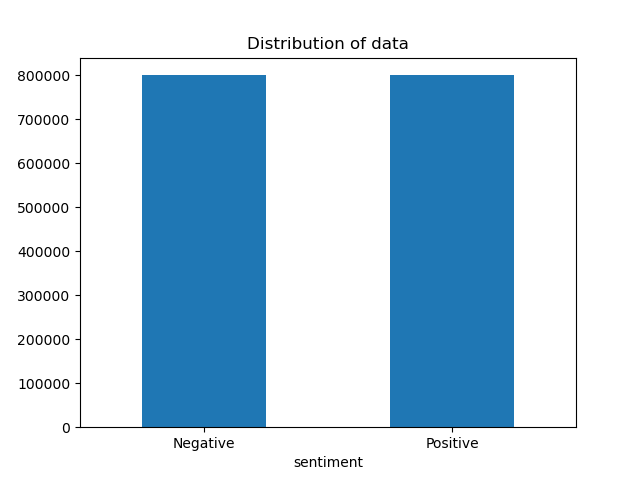
\includegraphics[width=0.6\textwidth]{figures/sentiment140-dataset-distribution.png}
            \caption{Classification distribution in the Sentiment140 dataset.}
        \end{figure}
        \FloatBarrier

        Further examination of the dataset can be accomplished by extracting a positively and negatively classified entry, the dataset provides six features for each post: Target (the sentiment polarity), ID, Date, Flag (the query), User, and Text (the body).

        \FloatBarrier
        \begin{table}[h]
            \centering
            \caption{Example of a positive post.}
            \label{tbl:positive_post}
            \begin{tabular}{p{0.15\linewidth} | p{0.6\linewidth}}
                Attribute & Value \\
                \hline\hline
                Target & 4 \\
                IDs & 1467822272 \\
                Date & Mon Apr 06 22:22:45 PDT 2009 \\
                Flag & NO\_QUERY \\
                User & ersle \\
                Text & I LOVE @Health4UandPets u guys r the best!! \\
            \end{tabular}
        \end{table}

        \begin{table}[h]
            \centering
            \caption{Example of a negative post.}
            \label{tbl:negative_post}
            \begin{tabular}{p{0.15\linewidth} | p{0.6\linewidth}}
                Attribute & Value \\
                \hline\hline
                Target & 0 \\
                IDs & 1467810369 \\
                Date & Mon Apr 06 22:19:45 PDT 2009 \\
                Flag & NO\_QUERY \\
                User & \_TheSpecialOne\_ \\
                Text & @switchfoot http://twitpic.com/2y1zl - Awww, that's a bummer.  You shoulda got David Carr of Third Day to do it. ;D \\
            \end{tabular}
        \end{table}
        \FloatBarrier

        \subsubsection{Pre-Processing the Data}
        Currently, the data is not fit for training purposes, to make it suitable the dataset must be cleaned up. Firstly, the dataset is loaded into a Pandas \pinline{DataFrame} using ISO-8859-1 encoding due to limitations with utf-8, then the unnecessary data can be removed from the dataset as it is loaded, as only the text and sentiment polarity are needed for training.

        \begin{python}
df = pd.read_csv(input_path, names=['sentiment', 'timestamp', 'datestring', 'N/A', 'user', 'text'], encoding='ISO-8859-1')
df = df[['text', 'sentiment']]
        \end{python}

        Next, the way sentiment is classified in the dataset must be changed; currently negative sentiment is labelled as `0' and positive is `4', this is changed to a simple binary classification where `0' is negative and `1' is positive.

        \begin{python}
df['sentiment'] = df['sentiment'].replace(4, 1)
        \end{python}

        The dataset should also be shuffled, this ensures that there are no related or similar tweets next to each other in the dataset.

        \begin{python}
toolkit.console("Shuffling dataset...")
df = df.sample(frac=1).reset_index(drop=True)
toolkit.console("Dataset shuffled.")
        \end{python}

        Now that the dataset has been prepared, the text of each post needs to be processed, for this purpose a class \pinline{TextProcessor} is defined to handle all processing.

        \begin{python}
class TextProcessor(object):
    def __init__(self):
        self.lemmatiser = WordNetLemmatizer()
        \end{python}
        
        The first function \pinline{preprocess()} is to remove various parts that will not contribute, or may even be detrimental, to the training of the model, such as urls, user mentions, etc. Firstly, several regex patterns are defined:

        \begin{python}
def preprocess(self, text: str) -> str:
    x_mention_pattern = r'@\S{4,}'
    ampersand_pattern = r'&amp;'
    url_pattern = r'((http://)[^ ]*|(https://)[^ ]*|( www\.)[^ ]*)'
    reddit_user_mention_pattern = r'/?u/\S+'
    reddit_sub_mention_pattern = r'/?r/\S+'
    newline_pattern = r'(\r\n|\r|\n)'
    reddit_url_match = r'/\[.*?(?=\]\((.*?)\))/g'
    reddit_url_replace = r'/\[.*?\]\(.*?\)/g'
        \end{python}

        Then \pinline{re.sub()} is called on the text for each substitution:

        \begin{python}
text = re.sub(x_mention_pattern, 'USER', text) # @user -> USER
text = re.sub(ampersand_pattern, '&', text) # &amp; -> &
text = re.sub(reddit_user_mention_pattern, 'USER', text) # /u/user or u/user -> USER
text = re.sub(reddit_sub_mention_pattern, 'SUBREDDIT', text) # /r/sub or r/sub -> SUBREDDIT
text = re.sub(url_pattern, 'URL', text) # https://link or http://link -> URL
text = re.sub(newline_pattern, ' ', text) # \\n -> ' '
        \end{python}

        Finally, for URLs on Reddit, which are in the format [shown text](URL hyperlink), all matches of Reddit's URL format are found, and replaced with just the text that would be shown to the user.

        \begin{python}
# Find all tags (text inside square brackets)
tags = [match.group(1) for match in re.finditer(r'\[(.*?)(?=\]\(.*?\))', text)]
# Replace all markdown links with the extracted tags
text = re.sub(r'\[.*?\]\(.*?\)', lambda match: tags.pop(0), text) # [name](link) -> name
        \end{python}

        There are also other optional functions that were experimented with for training in the \pinline{TextProcessor}: \pinline{lowercase()}, \pinline{lemmatise()}, and \pinline{soup()}, which toggle the text to lowercase, lemmatise and stem the text, and apply a \pinline{BeautifulSoup} html parser to the text, respectively.

        These functions are toggled off by default, but may be turned on by the user in settings. For further insight into these, visit the GitHub repository for the project \citep{sentimentanalysistool} (under \pinline{toolkit/data/preprocess.py}).

        \subsubsection{Training the Model}
        In the \pinline{BertModel}, a method \pinline{train()} for training the model is implemented, training on the Sentiment140 \citep{sentiment140dataset} dataset will fine-tune BERT to the specific linguistics and tone of social media. This function takes in a DataFrame containing the `text' and `sentiment' columns, along with the path to save the model to after training.

        \begin{python}
def train(self, dataset: pd.DataFrame, path: str) -> None:
        \end{python}

        Firstly, the data must be split into training, testing, and validation data. This is accomplished by leveraging Scikit-learn's \pinline{train_test_split()} method twice, initially for an 80/20 train/test split, then once more for a 80/10/10 split for separate testing and validation sets, ensuring robust evaluation metrics.

        \begin{python}
X_train, X_test, y_train, y_test = train_test_split(text, sentiment, test_size=1 - train_ratio, stratify=sentiment, random_state = 42)
X_val, X_test, y_val, y_test = train_test_split(X_test, y_test, test_size=test_ratio/(test_ratio + val_ratio), stratify=y_test, random_state=42)
        \end{python}

        After this, \pinline{self.model} and \pinline{self.tokeniser} are re-initialised to avoid interference from any previously stored configurations. Then the data is encoded using \pinline{self.tokenise()} to transform the text inputs into token IDs.

        \begin{python}
self.tokeniser = BertTokenizer.from_pretrained('bert-base-uncased', do_lower_case=True)
self.model = TFBertForSequenceClassification.from_pretrained('bert-base-uncased', num_labels=2)
        \end{python}

        Each value is encoded using \pinline{self.tokenise()} which takes a string `text' to transform the text inputs into token IDs.

        \begin{python}
self.tokeniser.batch_encode_plus(text, padding=True, truncation=True, max_length=128, return_tensors='tf') 
        \end{python}

        Following this, \pinline{self.fit_model()} is called, the model is compiled with an optimiser, loss function, and evaluation metrics. The Adam optimiser is used with a learning rate of 2e-5, and a sparse categorical cross-entropy loss function is defined to compute the difference between predicted and actual labels, with accuracy chosen as the evaluation metric for assessing model performance.

        \begin{python}
optimiser = tf.keras.optimizers.Adam(learning_rate=2e-5)
loss = tf.keras.losses.SparseCategoricalCrossentropy(from_logits=True)
metric = tf.keras.metrics.SparseCategoricalAccuracy('accuracy')
self.model.compile(optimizer=optimiser, loss=loss, metrics=[metric])
        \end{python}

        Finally, the model is fitted to the encoded data using \pinline{self.model.fit()}. This process trains the model on the training data while simultaneously validating its performance on the validation set. The batch size, which is the number of samples processed per gradient update, is set to 32, and the training process iterates over the dataset for 3 epochs.

        Through these iterations, the BERT model adapts its parameters to accurately classify the sentiment of the given social media post, enhancing its performance on this type of content.

        \begin{python}
history = self.model.fit([X_train_encoded['input_ids'], X_train_encoded['token_type_ids'], X_train_encoded['attention_mask']], np.array(y_train), validation_data=([X_val_encoded['input_ids'], X_val_encoded['token_type_ids'], X_val_encoded['attention_mask']], np.array(y_val)), batch_size=32, epochs=3)
        \end{python}

        \subsubsection{Cross-Validation}
        Cross-validation is a crucial element to evaluate the performance and robustness of a machine learning model. By splitting the dataset into multiple folds, cross-validation ensures that the model generalises well for unseen data, reducing the likelihood of overfitting, while also providing insight into the model's consistency across different subsets of data.

        This method is called at the end of the \pinline{train()} function instead of the single \pinline{self.fit_model()} call, if the user has enabled cross-validation. It takes in the training \pinline{DataFrame} and the number of splits \pinline{n_splits}, which defaults to 5. The text and sentiment columns of the dataset are converted into lists to be used later.

        \begin{python}
def cross_validate(self, dataset: pd.DataFrame, n_splits: int = 5) -> None:
    text = dataset['text'].tolist()
    sentiment = dataset['sentiment'].tolist()
        \end{python}

        Scikit-learn's \pinline{KFold} class is used to create cross-validation splits, shuffling the data before splitting to randomise the data.

        \begin{python}
kf = KFold(n_splits=n_splits, shuffle=True, random_state=42)
        \end{python}

        After initialising several empty lists for test loss, test accuracy, train accuracy, predicted labels, and actual labels, the function enters a loop which iterates through each fold; every iteration splits the data into training and validation sets, tokenises them, then fits and tests the model.

        \begin{python}
for train_index, val_index in kf.split(text):
    X_train, X_val = [text[i] for i in train_index], [text[i] for i in val_index]
    y_train, y_val = [sentiment[i] for i in train_index], [sentiment[i] for i in val_index]
    X_train_encoded = self.tokenise(X_train)
    X_val_encoded = self.tokenise(X_val)
    history = self.fit_model(X_train_encoded, y_train, X_val_encoded, y_val)
    test_loss, test_accuracy, pred_labels, actual_labels = self.test(X_val_encoded, y_val)
        \end{python}

        The results of each fold are appended to their corresponding, predefined lists for further analysis.

        \subsubsection{Testing the Model}
        In order to evaluate the model's performance on unseen data, it must be tested. This is done through the \pinline{test()} method, which takes the encoded test data in the form of a dictionary, and their corresponding labels in a list. The function returns key metrics such as test loss, test accuracy, and the predicted labels; these metrics help assess how well the model has generalised from the training data to the test data.

        \begin{python}
def test(self, X_test_encoded: dict, y_test: list[int]) -> tuple[float, float, list[str], list[str]]:
        \end{python}

        The model is evaluated on the test data using the \pinline{self.model.evaluate()} method.

        \begin{python}
test_loss, test_accuracy = self.model.evaluate([X_test_encoded['input_ids'], X_test_encoded['token_type_ids'], X_test_encoded['attention_mask']], np.array(y_test))
        \end{python}

        Then predictions are made using the \pinline{self.model.predict()} method, which returns logits. Using TensorFlow's \pinline{argmax()} function, the predicted labels can be obtained, which are then converted to a NumPy array and then their sentiment as a string using list comprehensions.

        \begin{python}
pred = self.model.predict([X_test_encoded['input_ids'], X_test_encoded['token_type_ids'], X_test_encoded['attention_mask']])
logits = pred.logits
pred_labels = tf.argmax(logits, axis=1)
pred_labels = pred_labels.numpy()
labels = {1: 'Positive', 0: 'Negative'}
pred_labels = [labels[i] for i in pred_labels]
actual_labels = [labels[i] for i in y_test]
        \end{python}

    \subsection{Predictions}
    The \pinline{predict()} function is designed to leverage the batch-processing and parallel-processing capabilities of BERT and TensorFlow, allowing for efficient sentiment prediction with a list of inputs of any length. It takes a list of strings to analyse, and returns the predicted sentiment labels for each input string.

    \begin{python}
def predict(self, text: list[str]) -> list[str]:
    \end{python}

    Initially, the input text is tokenised using the \pinline{self.tokenise()} method, which encodes the text into input IDs, token type IDs, and attention masks. These encoded values are then passed to the \pinline{self.model.predict()} function to get the predictions.

    \begin{python}
input_ids, token_type_ids, attention_mask = self.tokenise(text).values()
prediction = self.model.predict([np.array(input_ids), np.array(token_type_ids), np.array(attention_mask)])
    \end{python}

    Next, the prediction logits are processed to obtain the probability distributions over the classes using TensorFlow's \pinline{softmax()} function, and the confidence for each prediction is determined by the maximum probability value.

    \begin{python}
pred_logits = prediction.logits
pred_probs = tf.nn.softmax(pred_logits, axis=1).numpy()
pred_confidence = np.max(pred_probs, axis=1)
    \end{python}

    Finally, the predicted labels are determined using TensorFlow's \pinline{argmax()} function on the logits. The labels are mapped to their corresponding sentiment labels `Positive' or `Negative'. However, if the confidence score of a prediction is less than the threshold defined by the user, it is labelled as `Neutral'.

    \begin{python}
labels = {1: 'Positive', 0: 'Negative'}
pred_label_indices = np.argmax(pred_logits, axis=1)
pred_labels = [labels[i] if confidence >= confidence_threshold else 'Neutral' for i, confidence in zip(pred_label_indices, pred_confidence)]
    \end{python}

    The function then returns the predicted labels for further analysis.

\section{Social Media Data Collection}
The following section details the methods used to collect data from social media platforms for sentiment analysis. The data collection functionality is implemented within the \pinline{XScraper} and \pinline{RedditScraper} classes in \pinline{toolkit/data/social.py}. Unfortunately, due to new limitations with the free version of the X API which prevent searching posts, the \pinline{XScraper} class is not fully implemented and will be excluded from this section.

The \pinline{RedditScraper} class is used to scrape post data from Reddit, including comments if the user's configuration calls for it, using the PRAW library. It interfaces with Reddit's API to retrieve data based on specified subreddits and search terms.

Firstly, the class initialises by setting up an instance of the Reddit API \pinline{praw.Reddit}. In this method, the necessary credentials are fetched (client ID, client secret, and user agent) from the environment variables. Storing these as environment variables prevents them from being hard-coded, increasing security and allows flexibility between users.

\begin{python}
class RedditScraper(object):
    def __init__(self):
            self.api = praw.Reddit(client_id=os.getenv('REDDIT_CLIENT_ID'), client_secret=os.getenv('REDDIT_CLIENT_SECRET'), user_agent=os.getenv('REDDIT_USER_AGENT'))
\end{python}

Next, the class defines the \pinline{search_subs()} method, which is designed to search Reddit for posts and comments across any number of subreddits based on a list of given search terms. It takes a dictionary \pinline{subs} where the keys are the subreddits to search and the values are lists of search terms, and an integer \pinline{n}, which is the number of posts to retrieve per subreddit. Then it returns either a single \pinline{DataFrame} containing the scraped posts, or a tuple of two \pinline{DataFrame}s, containing both scraped posts and comments.

\begin{python}
def search_subs(self, subs: dict[str, list[str]], n: int = 10) -> 'pd.DataFrame | tuple[pd.DataFrame, pd.DataFrame]':
\end{python}

Initially, the function defines two empty lists \pinline{posts} and \pinline{comments}, it then iterates through the given dictionary's key/value pairs, calling \pinline{self.search_sub()} on them and storing the returned values in temporary lists; these are then concatenated with the main lists before moving on to the next iteration.

\begin{python}
posts = []
comments = []
for sub, search_terms in subs.items():
    temp_posts, temp_comments = self.search_sub(sub, search_terms, n)
    posts += temp_posts
    comments += temp_comments
\end{python}

As the Reddit API returns \pinline{Submission} and \pinline{Comment} objects, the function must now extract the needed attributes from these objects. To do this, two lists \pinline{post_attributes} and \pinline{post_comments} are created to be two dimensional lists. The function then iterates through the list of posts, initialising a list \pinline{post_comments}, and checks \pinline{post.is_self} to make sure the post is text-only. If it is, certain attributes are pulled from the \pinline{Submission} object:

\begin{itemize}
    \item \pinline{id}: ID of the submission.
    \item \pinline{subreddit.display_name}: Provides an instance of \pinline{Subreddit} and then retrieves the name of that subreddit.
    \item \pinline{created_utc}: The time the submission was created, represented in Unix Time. 
    \item \pinline{title}: The title of the submission.
    \item \pinline{selftext}: The body text of the submission.
    \item \pinline{score}: The number of `upvotes' for the submission.
\end{itemize}

Also, while not an attribute of \pinline{Submission}, the tuple \pinline{tuple(comment for comment in post_comments)} is created as a list of comment IDs and added, with the other attributes, to a row in \pinline{post_attributes}.

\begin{python}
for post in posts:
    post_comments = []
    if post.is_self:
        if scrape_comments:
            # Functionality will be covered next
        post_attributes.append([post.id, post.subreddit.display_name, post.created_utc, post.title, post.selftext, post.score, tuple(comment for comment in post_comments)])
\end{python}

If scraping comments is enabled by the user, this will also iterate over the comments of the post, pulling the same attributes as it did for the post, but along with the \pinline{submission.id} of the comment, referring to the parent post.

\begin{python}
for comment in comments[posts.index(post)]:
    post_comments.append(comment.id)
    comment_attributes.append([comment.id, comment.submission.id, comment.subreddit.display_name, comment.created_utc, comment.body, comment.score])
\end{python}

Finally, the function defines column labels for the post and comment attributes, and adds them to \pinline{posts_df} and \pinline{comments_df}, returning the resulting \pinline{DataFrame}s.

\begin{python}
columns = ['ID', 'Subreddit', 'Date/Time', 'Title', 'Body', 'Score', 'Comments']
posts_df = pd.DataFrame(post_attributes, columns=columns)
if scrape_comments: 
    columns = ['ID', 'PostID', 'Subreddit', 'Date/Time', 'Body', 'Score']
    comments_df = pd.DataFrame(comment_attributes, columns=columns)
\end{python}

The function \pinline{search_sub()}, which is called in \pinline{search_subs()}, searches Reddit for posts and comments within a specified subreddit based on the given search terms (none if the list is empty). It's parameters are the subreddit's name, the search terms to query, and the amount of posts to collect, returning a list of posts and comments.

\begin{python}
def search_sub(self, sub: str, search_terms: list[str], n: int = 10) -> tuple[list, list]:
\end{python}

It then iterates over the search terms, requesting posts that contain the query in the specified subreddit, and adds the received post to the \pinline{posts} list. If comment scraping is enabled, it calls \pinline{self.search_comments()}, passing the post as an argument, and adds the returned list to the \pinline{comments} list.

\begin{python}
if search_terms:
    for search_term in search_terms:
        for post in self.api.subreddit(sub).search(search_term):
            posts.append(post)
            if scrape_comments:
                post.comment_sort = 'hot'
                comments.append(self.search_comments(post))
\end{python}

If \pinline{search_terms} is empty, a near identical code block is executed, the difference being that it only has one iteration over the top ten posts in the subreddit after sorting by `hot'.

\begin{python}
for post in self.api.subreddit(sub).hot(limit=n):
# Rather than `for post in self.api.subreddit(sub).search(search_term):'
\end{python}

The final function in \pinline{RedditScraper} is \pinline{search_comments()}. This method takes arguments \pinline{post} and \pinline{limit}, being the parent post and the amount of comments to retrieve respectively. This function simply iterates over the \pinline{CommentForest} returned by \pinline{post.comments}, and adds the results to a list of comments to be returned.

\begin{python}
def search_comments(self, post, limit: int = 5) -> list:
post_comments = []
    post.comment_limit = limit
    post.comments.replace_more(limit=0) # Remove all MoreComments
    for comment in post.comments:
        post_comments.append(comment)
    return post_comments
\end{python}

\section{Database Management}
All management of the database is done within the \pinline{PostCollector} class found in \pinline{toolkit/data/database.py}. This class incorporates the functionality of \pinline{BertModel}, \pinline{RedditScraper}, and database management operations defined in the class itself.

The class initialises with the passed arguments \pinline{model} and \pinline{scraper}, an instance of \pinline{BertModel} and \pinline{RedditScraper} respectively, and a \pinline{profile}, which is a dictionary containing the details of subreddits and search terms to be scraped. \pinline{self.path} is then set to point at a directory based on the profile ID, which is where the collected data will be stored in \pinline{.json} format. Finally, two empty \pinline{DataFrame}s are created with the relevant column labels for posts and comments, and the object calls \pinline{self.from_json()} to load any data that may already exist for this profile.

\begin{python}
class PostCollector(object):
    def __init__(self, model, scraper, profile: dict[str, any]) -> None:
        self.model = model
        self.scraper = scraper
        self.profile = profile
        self.path =f'{toolkit.get_dir()}/src/profiles/{self.profile["id"]}'
        self.posts = pd.DataFrame(columns=['ID', 'Subreddit', 'Date/Time', 'Title', 'Body', 'Score', 'Comments', 'Sentiment'])
        self.comments = pd.DataFrame(columns=['ID', 'PostID', 'Subreddit', 'Date/Time', 'Body', 'Score', 'Sentiment'])
        self.from_json()
\end{python}

The \pinline{scrape_posts()} method is responsible for collecting data from the subreddits and search terms configured in the loaded profile. It collects and processes posts and comments, cleans the text, predicts sentiment, and stores the data in the database.

Firstly, it initialises an instance of the \pinline{TextProcessor} object for later, and retrieves the subreddits to be scraped from \pinline{self.profile}. Then it calls \pinline{search_subs()} to retrieve posts and or comments using the \pinline{RedditScraper} depending on the current configuration; the resulting data is stored in \pinline{new_posts} and or \pinline{new_comments}.

\begin{python}
def scrape_posts(self, n: int) -> None:
    text_processor = toolkit.TextProcessor()
    subs = self.profile['subs']
    if scrape_comments:
        new_posts, new_comments = self.scraper.search_subs(subs, n=n)
    else:
        new_posts = self.scraper.search_subs(subs, n=n)
\end{python}

Next, the method iterates over each post ID in \pinline{new_posts} to get the title and body of each one using \pinline{self.get_record()}, which returns the specific record from a \pinline{DataFrame} for the given ID and column. If the title or body is \pinline{None}, then the row is dropped from \pinline{new_posts}, otherwise the title and body are cleaned with the \pinline{TextProcessor} and concatenated with a BERT separator token \pinline{'[SEP]'}.

\begin{python}
for ID in new_posts['ID']:
    title = self.get_record(new_posts, ID, 'Title')
    body = self.get_record(new_posts, ID, 'Body')
    if title is None or body is None:
        index = new_posts.index[new_posts['ID'] == ID]
        new_posts.drop(index)
        continue
    title = text_processor.clean(title)
    body = text_processor.clean(body)
    text = f"{title} [SEP] {body}"
    if not text.strip():
        print(f"Empty text for post ID: {ID}")
    else:
        all_texts.append(text)
\end{python}

All non-empty concatenated texts are then added to a list for batch sentiment prediction through \pinline{BertModel}'s \pinline{predict()} method, and once the sentiment is analysed, these values are inserted as a column into \pinline{new_posts}. Finally, \pinline{new_posts} is added to \pinline{self.posts}, removing any duplicate posts to ensure the integrity of the data.

\begin{python}
post_sentiments = self.model.predict(all_texts)
new_posts.insert(6, 'Sentiment', post_sentiments, True)
self.posts = pd.concat([self.posts, new_posts], ignore_index=True)
self.posts.drop_duplicates(keep='last', inplace=True)
self.posts.drop_duplicates('ID', keep='last', inplace=True)
\end{python}

If comment search is enabled, there is similar behavior, the only difference is that the title and body of the parent post are concatenated with the body of the comment using the same BERT separator tokens. This allows BERT to predict the sentiment of the comment with the context of the parent post.

\begin{python}
for ID in new_comments['ID']:
    post_id = self.get_record(new_comments, ID, 'PostID')
    # Get records of post title, body, and comment
    if title is None or body is None:
        # Drop as before
    # Clean the texts
    text = f"{title} [SEP] {body} [SEP] {comment}"
\end{python}

The new data is then stored in \pinline{.json} format for later use using \pinline{self.to_json()}.

\section{Data Visualisation}
The \pinline{Analyser} class in \pinline{toolkit/analysis/analyse.py} is crucial for interpreting sentiment data to the user via visual representation; large datasets could be overwhelming to the user, so by visualising the data and breaking it up into more digestible formats, the user is able to make quicker and more accurate insights. Furthermore, representing the data graphically makes it far easier to spot patterns that are not immediately obvious when looking at raw data, such as the change in sentiment over time or comparisons between different subreddits or queries.

Upon initialisation, the \pinline{Analyser} class prepares the passed \pinline{DataFrame} by converting the sentiment labels into a numerical format with \pinline{self._set_sentiment_score()}, where `Positive', `Neutral', and `Negative' labels are converted to 1, 0, and -1 respectively. These new values are inserted as a new column, and if weighting by score is enabled in settings, these values are multiplied by the score (number of `upvotes') of the post; this allows the user to see how many people agree with each post, thus leading to a more in depth analysis. 

\begin{python}
class Analyser(object):
    def __init__(self, dataset: pd.DataFrame) -> None:
        self.dataset = dataset
        self._set_sentiment_score()

    def _set_sentiment_score(self) -> None:
        if toolkit.get_config('score_weighting'):
            self.dataset['SentimentScore'] = self.dataset['Score'] * self.dataset['Sentiment'].apply(self._sentiment_to_int)
\end{python}

This class defines three functions for chart creation, \pinline{generate_line()}, \pinline{generate_pie}, and \pinline{generate_bar}, for creating a line, pie, and bar chart respectively. They each take the \pinline{canvas} argument, which is a \pinline{FigureCanvas} object from \pinline{matplotlib} for use as a \pinline{QtPy} widget, along with a chart title, and start/end date for the plotted data. Both the line and bar chart also take the \pinline{labels} argument, which is a tuple containing the labels for the axis.

\begin{python}
def generate_line(self, canvas: FigureCanvas, title: str, labels: tuple[str, str], start_date: float, end_date: float) -> None:
def generate_pie(self, canvas: FigureCanvas, title: str, start_date: float = None, end_date: float = None) -> None:
def generate_bar(self, canvas: FigureCanvas, title: str, labels: tuple[str, str], start_date: float = None, end_date: float = None) -> None:
\end{python}

The line chart is useful for visualising the changes in sentiment score over a given time-frame; line charts can be useful for identifying trends such as seasonal variations, spikes, or declines in sentiment. This specific implementation also allows for data from different subreddits to be visualised separately as independently plotted lines, if \pinline{split_subs} is configured to do so.

\begin{figure}[h]
    \centering
    \begin{subfigure}{0.49\textwidth}
        \centering
        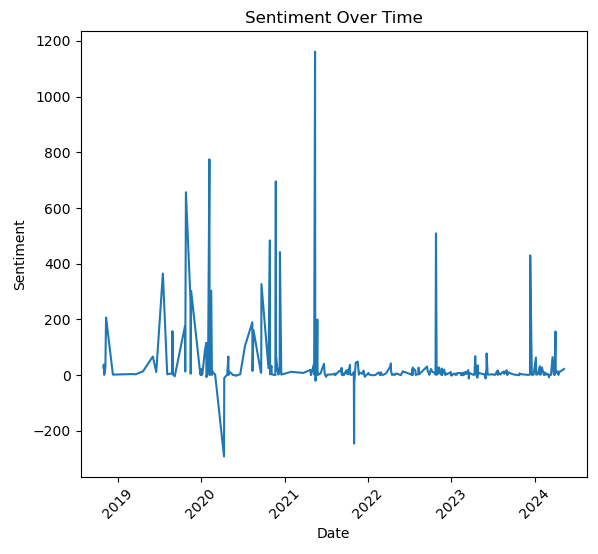
\includegraphics[width=\textwidth]{figures/line-chart.png}
    \end{subfigure}
    \begin{subfigure}{0.49\textwidth}
        \centering
        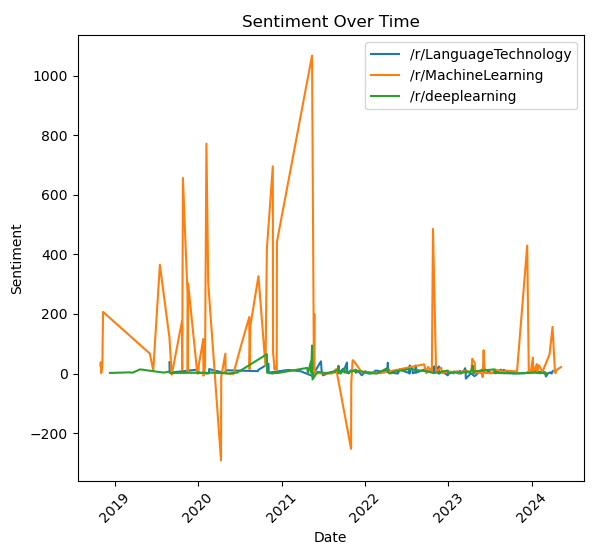
\includegraphics[width=\textwidth]{figures/split-line-chart.png}
    \end{subfigure}
    \caption{Example line charts with subreddit splitting enabled and disabled.}
\end{figure}

The pie chart represents the distribution of sentiment classifications within the dataset as a whole. Pie charts are great for showing the proportions of sentiment classes within the whole dataset, which makes them intuitive to the user, giving easy insight into which sentiment category dominates and how sentiment is distributed.

Finally, the bar chart compares the total sentiment scores across different subreddits. They are ideal for comparative analysis as they clearly display proportional quantities for different groups (in this case, subreddits),  allowing for clear visual indication of which subreddits and queries have the highest/lowest sentiment scores.

\begin{figure}[h]
    \centering
    \begin{subfigure}{0.49\textwidth}
        \centering
        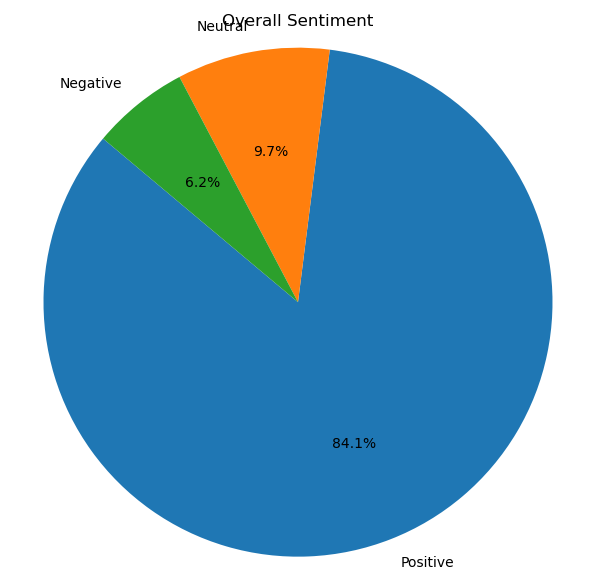
\includegraphics[width=\textwidth]{figures/pie-chart.png}
    \end{subfigure}
    \begin{subfigure}{0.49\textwidth}
        \centering
        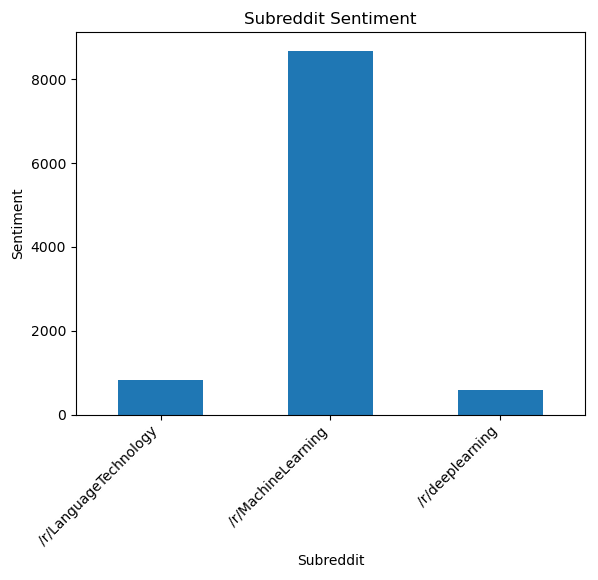
\includegraphics[width=\textwidth]{figures/bar-chart.png}
    \end{subfigure}
    \caption{Example pie and bar chart.}
\end{figure}

For further insight into the implementation of these charts, visit the GitHub repository \citep{sentimentanalysistool}.

\section{Graphical User Interface}

The GUI of the application (\pinline{toolkit/ui/interface.py}) serves as the means by which the user can interact with the functionality of the back-end processes. It is designed to provide an intuitive and user-friendly experience, while keeping performance and responsiveness to a high standard. This section outlines the architecture and components of the GUI, highlighting the core aspects such as the distinct windows and the use of parallel programming for long-running tasks. For the purpose of this application, the \pinline{QtPy} library was used, as it excels at creating complex, responsive, and user-friendly interfaces, as well as providing parallelism features.

    \subsection{Main Window}
    The \pinline{MainWindow} class, inheriting from \pinline{QtPy}'s \pinline{QMainWindow}, creates the main application, it displays widgets that link to the core functionalities of the program in an accessible format. The layout is built up by embedding other layouts and widgets within each other, creating an interface which is complex but pleasant to use. 

    \begin{figure}[h]
    \centering
        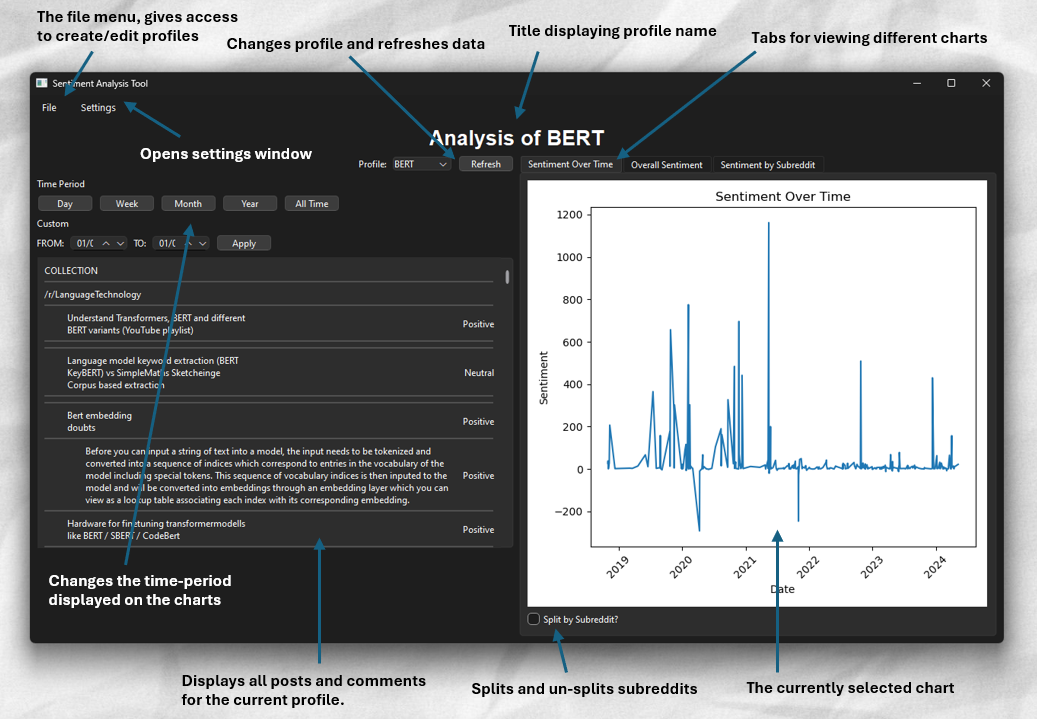
\includegraphics[width=0.95\textwidth]{figures/main-window-labels.png}
    \caption{The main window of the application.}
    \end{figure}

    As can be seen in the provided figure, the window consists of several main elements: a menu bar, a profile changer, a time period editor, a scrollable widget featuring all posts for the profile, and an area with tabs displaying different charts. Each distinct area is built up using layouts and widgets embedded in parent layouts, which are used as building blocks for the GUI. For example, the time period editor is built up through several different \pinline{MainWindow} methods, namely: 

    \begin{itemize}
        \item \pinline{self._make_time_period_layout()}
        \item \pinline{self._make_custom_time_layout()}
        \item \pinline{self._make_time_changer_layout()}
    \end{itemize}

    The time period layout consists of five buttons to change the time period to either the last twenty-four hours, week, month, year, or all-time.

    The \pinline{QtPy} object \pinline{QHBoxLayout} is used to create a layout consisting of a row of horizontal `boxes', which are used for placing widgets (or other layouts) into. Due to the one-dimensional layout of this, it is necessary to embed layouts \pinline{QHBoxLayout} and \pinline{QVBoxLayout} within each other to achieve a complex GUI. Once the layout is created, a \pinline{QPushButton} widget is created, connected to the \pinline{self._time_period_day()} function, and added to the layout as such (code reduced for simplicity):

    \begin{python}
def _make_time_period_layout(self):
    layout = QHBoxLayout()
    button_day = QPushButton("Day")
    button_day.clicked.connect(self._time_period_day)
    layout.addWidget(button_day)
    layout.addStretch()
    return layout
    \end{python}

    Following this, another layout is created to enable the user to select a more specific time period using selection boxes. This layout is implemented in a similar way, however, to prevent the charts updating every time the user increments or decrements the start/end date, a button labelled `Apply' is also added. For this button to work and pass the new start/end date to its connected function, a lambda function must be created as the passed function.

    \begin{python}
def _make_custom_time_layout(self):
    layout = QHBoxLayout()
    selector_from = QDateEdit()
    selector_to = QDateEdit()
    apply = QPushButton("Apply")
    apply.clicked.connect(lambda: self._set_dates(selector_from, selector_to))
    # Add widgets and return layout
    \end{python}

    These are then added to their parent layout, itself being a child of other layouts.

    \begin{python}
def _make_time_changer_layout(self):
    layout = QVBoxLayout()
    time_period_layout = self._make_time_period_layout() 
    custom_time_layout = self._make_custom_time_layout() 
    layout.addLayout(time_period_layout)
    layout.addLayout(custom_time_layout)
def _make_left_layout(self):
    layout.addLayout(self._make_time_changer_layout())
def _make_main_layout(self):
    layout.addLayout(self._make_left_layout())
    \end{python}

    Finally, the finished layout, made up of dozens of child layouts and widgets, is set as the layout of the window itself in \pinline{MainWindow.__init__()}.

    \begin{python}
class MainWindow(QMainWindow):
    def __init__(self, *args, **kwargs):
        self.widget = QWidget(self)
        self.setCentralWidget(self.widget)
        self.layout = self._make_layout()
        self.widget.setLayout(self.layout)  
    \end{python}

    To see the \pinline{MainWindow} in full detail, see the GitHub \citep{sentimentanalysistool}.

    \subsection{Profile Editor}
    The \pinline{ProfileEditorWindow} is a dedicated interface for managing the brand profiles. It allows the user to create, edit, and delete profiles; each profile contains information about which subreddits to monitor and analyse, and which search terms, if any, to query.

    \begin{figure}[h]
        \centering
            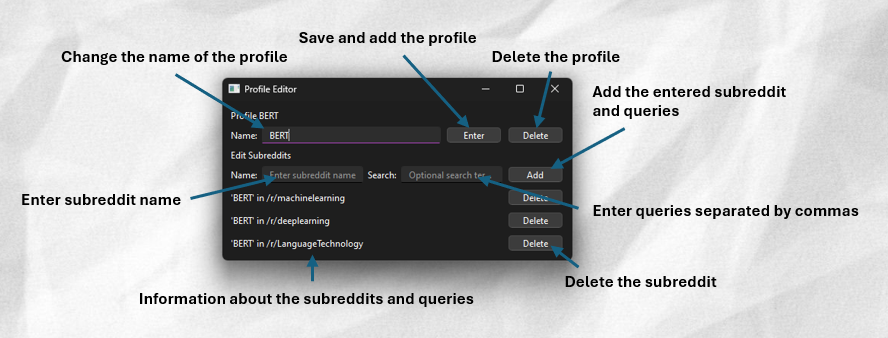
\includegraphics[width=0.95\textwidth]{figures/profile-editor-window-labels.png}
        \caption{The profile editor window.}
    \end{figure}

    In order for this window to communicate with the main window, a \pinline{pyqtSignal} object must be defined, which allows the transmission of signals between different objects in a program. This signal object is then used in the \pinline{ProfileEditorWindow._update()} function to \pinline{emit()} a signal that is picked up by the \pinline{MainWindow}. This allows the main window to update every time the profile editor window does.

    \begin{python}
class ProfileEditorWindow(QWidget):
    submit_clicked = pyqtSignal()
    def _update(self):
        self.submit_clicked.emit()

# Inside MainWindow
self.window_profile_editor.submit_clicked.connect(self._update)
    \end{python}

    To gain more insight into the workings of the \pinline{ProfileEditorWindow}, please refer to the GitHub repository \citep{sentimentanalysistool}.

    \subsection{Settings}
    The \pinline{SettingsWindow} class allows the user to customise various settings and preferences. It is divided into several distinct tabs for organisation and ease of use, such as General, Analysis, Personalisation, etc.

    \begin{figure}[h]
        \centering
            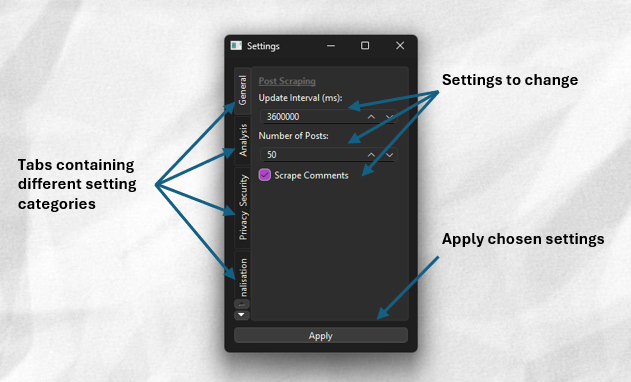
\includegraphics[width=0.95\textwidth]{figures/settings-window-labels.png}
        \caption{The profile editor window.}
    \end{figure}
    
    \begin{itemize}
        \item \textbf{General}: user can change the update interval, number of posts to scrape, and toggle comment scraping.
        \item \textbf{Analysis}: provides options for text processing such as lowercase, lemmatisation, and \pinline{BeautifulSoup} parsing, as well as model configurations like toggling cross-validation and changing the confidence threshold.
        \item \textbf{Privacy \& Security}: settings such as encryption can be toggled here (no functionality implemented).
        \item \textbf{Personalisation}: allows the user to customise the appearance of the application, such as font, colour, and chart styling (no functionality implemented).
        \item \textbf{Export \& Sharing}: allows the user to initiate a data export or share analyses (no functionality implemented).
        \item \textbf{Feedback \& Support}: provides the user with links to the creator's LinkedIn profile, send the creator an email, or visit the codebase on GitHub.
    \end{itemize}

    Each of these tabs have their own unique settings, for example, in the `General' tab, the update interval can be set using a \pinline{QSpinBox} that sets the interval in milliseconds, allowing a range anywhere from one second to twenty-four hours.

    \begin{python}
update_interval_spinbox = QSpinBox()
update_interval_spinbox.setMinimum(1000)
update_interval_spinbox.setMaximum(86400000)
update_interval_spinbox.setValue(toolkit.get_config("update_interval"))
update_interval_spinbox.valueChanged.connect(lambda value, name="update_interval": self._update_setting(name, value))
    \end{python}

    To prevent constant updates to the \pinline{MainWindow}, all settings changes are deferred inside of the \pinline{self.settings} dictionary until the user clicks the `Apply' button.

    \begin{python}
def _update_setting(self, name, value):
    self.settings[name] = value
    \end{python}

    This window uses similar functionality as the \pinline{ProfileEditorWindow} to communicate with the \pinline{MainWindow} using a \pinline{pyqtSignal} object, which this time is sent when the user clicks `Apply' and \pinline{self._apply_settings()} is called.

    \begin{python}
class SettingsWindow(QWidget):
    submit_clicked = pyqtSignal()
    def _apply_settings(self):
        for setting_name, value in self.settings.items():
            toolkit.set_config(setting_name, value)
        self.submit_clicked.emit()
    \end{python}

    \subsection{Parallelism for Long-Running Tasks}
    To ensure the application runs smoothly and efficiently, specifically during resource-intensive tasks such as social media scraping and analysis, \pinline{QtPy}'s parallelism features are used. Running tasks in parallel allows the application to perform multiple tasks simultaneously, significantly reducing the time required to execute. It is also ensures that the GUI stays responsive during these tasks rather than freezing, meaning the user can continue to interact with and use the program unimpeded.

    In the \pinline{MainWindow}, parallelism is employed in the execution of two functions: \pinline{self._collect_new_posts()} and \pinline{self._train_model()}, both of which are long-running tasks which would freeze the application for an undesirably extended period of time without parallelism. Initially, the class defines a \pinline{self.threadpool} storing a \pinline{QtPy.QThreadPool} object, which handles the queuing and execution of `workers'.

    \begin{python}
class MainWindow(QMainWindow):
    def __init__(self, *args, **kwargs):
        self.threadpool = QThreadPool()
    \end{python}

    To be able to use the \pinline{QThreadPool}, a new class \pinline{Worker} is defined, inheriting from \pinline{QtPy.QRunnable}, with the function to execute passed as an argument to it's \pinline{run()} method, using the \pinline{@pyqtSlot()} decorator.

    \begin{python}
class Worker(QRunnable):
    def __init__(self, fn: callable, *args, **kwargs) -> None:
        super(Worker, self).__init__()
        self.fn = fn
        self.signals = WorkerSignals()
    @pyqtSlot()
    def run(self):
        try:
            result = self.fn(*self.args, **self.kwargs) # Execute the passed function
        except: # Emit exception
        else:
            self.signals.result.emit(result)
        finally:
            self.signals.finished.emit()
    \end{python}

    Finally, the two long-running functions are called using multithreading by passing them as a callable upon a \pinline{Worker} creation. The program starts the worker and waits for the `finished' signal from to be emitted, so that it can call \pinline{self._update()}.

    \begin{python}
def _collect_new_posts(self):
    worker = Worker(lambda: self.collector.scrape_posts(toolkit.get_config('n_posts')))
    worker.signals.finished.connect(self._update)
    self.threadpool.start(worker)

def _train_model(self):
    worker = Worker(self.model.train)
    worker.signals.finished.connect(self._update)
    self.threadpool.start(worker)
    \end{python}

\chapter{Results \& Discussion}
The implementation and testing of the sentiment analysis tool \citep{sentimentanalysistool} have yielded valuable insights into the functionality and performance of the developed software. The purpose of this chapter is to present a software evaluation, encompassing the evaluation of key components of the system, such as sentiment analysis, social media interfacing, data management, and the GUI. Furthermore, it discusses the details of fulfillment for the previously outlined functional and non-functional requirements of the application from the requirements analysis, followed by further reflection on the development process and possible areas for improvement.

\section{Software Evaluation}
    \subsection{Sentiment Analysis Model}
    The sentiment analysis model is the core component of the application, aimed at classifying the sentiment of social media posts into positive, and negative categories. While PFDualBERT was not implemented, BERT saw great success in terms of accuracy and other metrics.

    Initially BERT model was trained on a dataset containing 1,600,000 rows over 3 epochs and with a learning rate of 2e-5. This proved successful according to the predefined requirements of this project, showing accuracy of 86.95\% during testing. However, the model took 48,755 seconds to complete training, along with a further 519 seconds of testing; this is entirely impractical as this inhibits further fine-tuning that may take place. The training also showed over-fitting taking place, as the training accuracy skyrocketed up to nearly 90\% over each epoch while validation accuracy hovered at ~87\%.

    \FloatBarrier
    \begin{figure}[h]
        \centering
        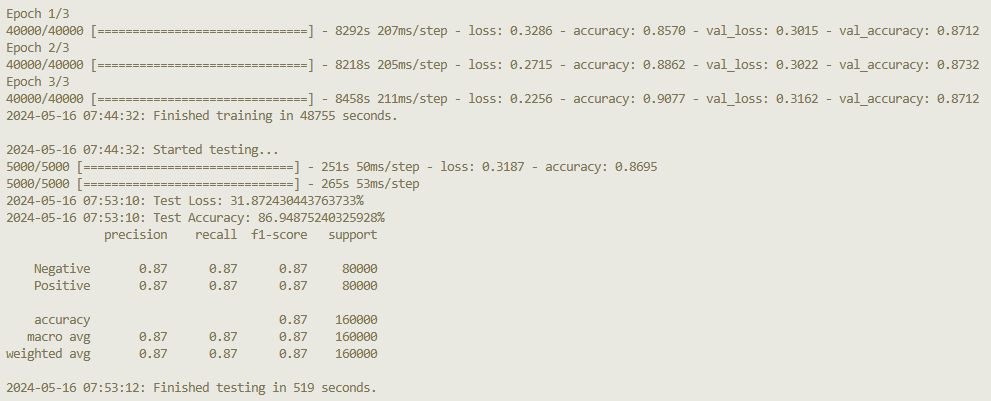
\includegraphics[width=0.95\textwidth]{figures/train-16m-console.png}
        \caption{Standard training results on 1.6 million rows.}
    \end{figure}

    \begin{figure}[h]
        \centering
        \begin{subfigure}{0.49\textwidth}
            \centering
            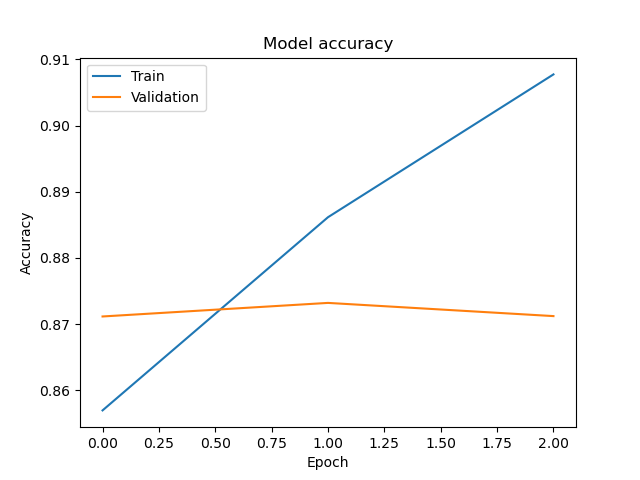
\includegraphics[width=\textwidth]{figures/standard-train-1600000-accuracy.png}
        \end{subfigure}
        \begin{subfigure}{0.49\textwidth}
            \centering
            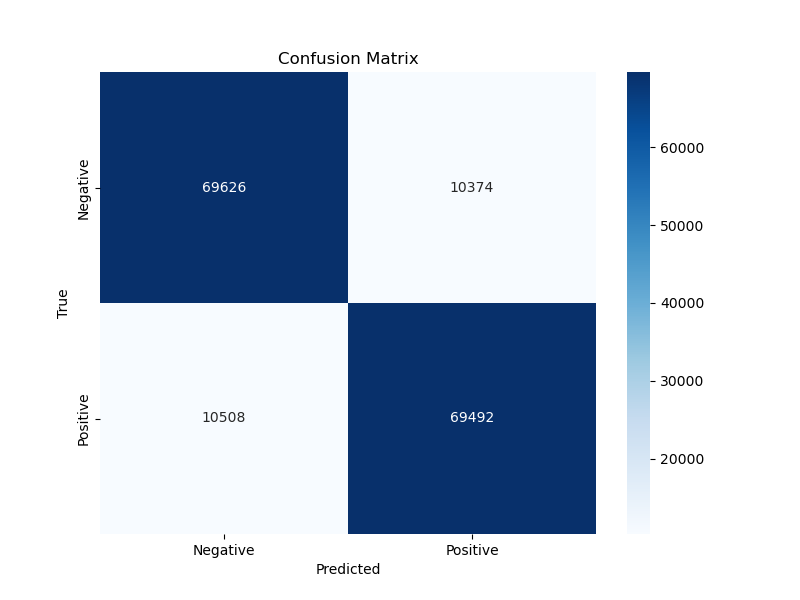
\includegraphics[width=\textwidth]{figures/standard-train-1600000-confusion.png}
        \end{subfigure}
        \caption{Accuracy and confusion matrix for standard training on 1.6 million rows.}
    \end{figure}
    \FloatBarrier

    To combat this, the model was trained using cross-validation with 5 folds and only 5,000 rows of training data. This approach showed great success, proving to have an accuracy of 99.9\% during testing, corresponding train/test accuracy, and only one false positive and one false negative. This conveys that the cross-validation dramatically improved the accuracy and generalisation of the model. It also proved to be significantly faster than training on the full dataset; however, when attempting to train on 10,000 rows, an Out-Of-Memory (OOM) error was thrown, showing that this method uses a large amount of resources when compared to standard training.

    \FloatBarrier
    \begin{figure}[h]
        \centering
        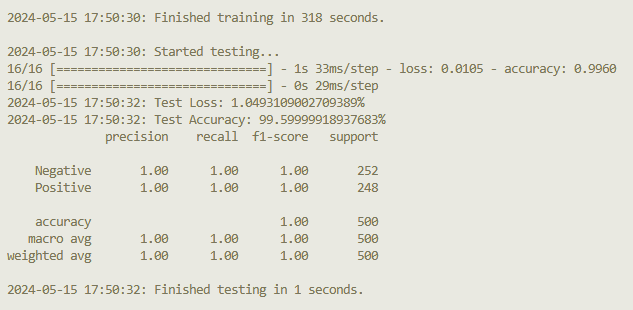
\includegraphics[width=0.95\textwidth]{figures/cross_validation_5000_overall.png}
        \caption{Training results using 5 fold cross-validation on 5,000 rows.}
    \end{figure}

    \begin{figure}[h]
        \centering
        \begin{subfigure}{0.49\textwidth}
            \centering
            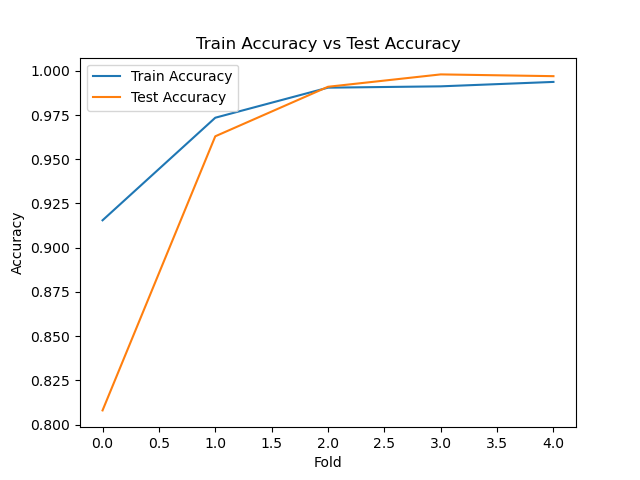
\includegraphics[width=\textwidth]{figures/cross_validation_5000_accuracy.png}
        \end{subfigure}
        \begin{subfigure}{0.49\textwidth}
            \centering
            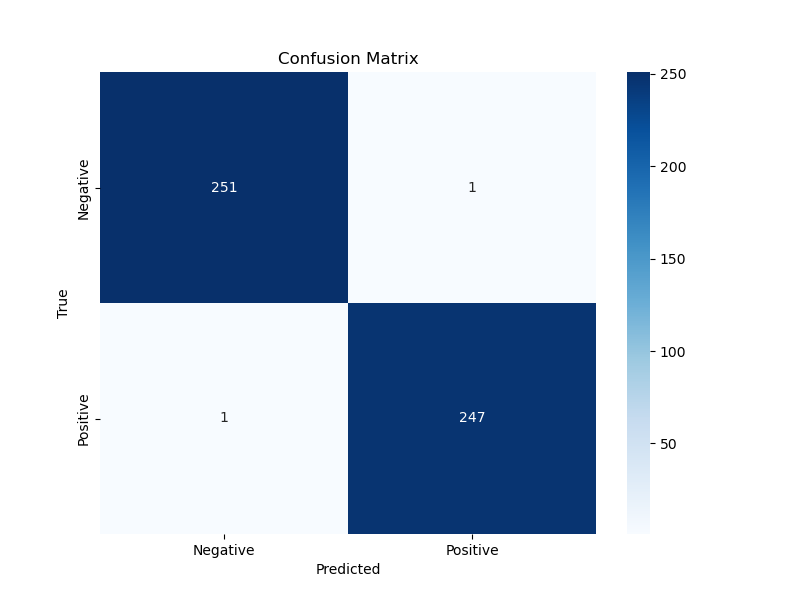
\includegraphics[width=\textwidth]{figures/cross_validation_5000_confusion.png}
        \end{subfigure}
        \caption{Accuracy and confusion matrix for 5 fold cross-validation on 5,000 rows.}
    \end{figure}
    \FloatBarrier

    Finally, an attempt was made at using 3 fold cross-validation with more rows, and it was found that this approach allows training on a dataset of up to 100,000 rows (higher was not attempted). It was found that even with the extra training data, performance actually showed a fractional decrease, with an accuracy of 99.49\%, mainly as there was not much room to improve. This decrease in accuracy should be disregarded due to the many variables at play, however the training execution time should not be ignored; the time taken for this approach was 4,975 seconds, a 93.61\% increase compared to the 318 seconds that the previous approach took, meaning that even though this may increase generalisation, it is entirely inefficient in comparison.

    \FloatBarrier
    \begin{figure}[h]
        \centering
        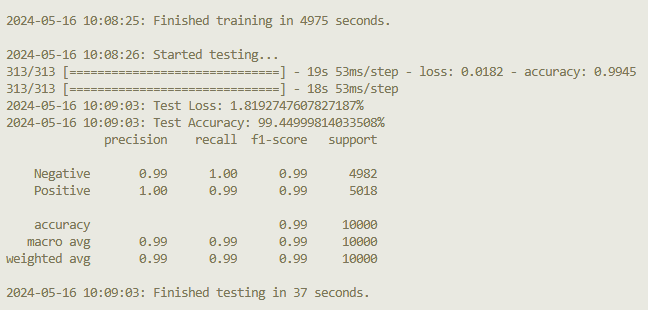
\includegraphics[width=0.95\textwidth]{figures/cross_validation_100000_console_overall_3f.png}
        \caption{Training results using 3 fold cross-validation on 100,000 rows.}
    \end{figure}

    \begin{figure}[h]
        \centering
        \begin{subfigure}{0.49\textwidth}
            \centering
            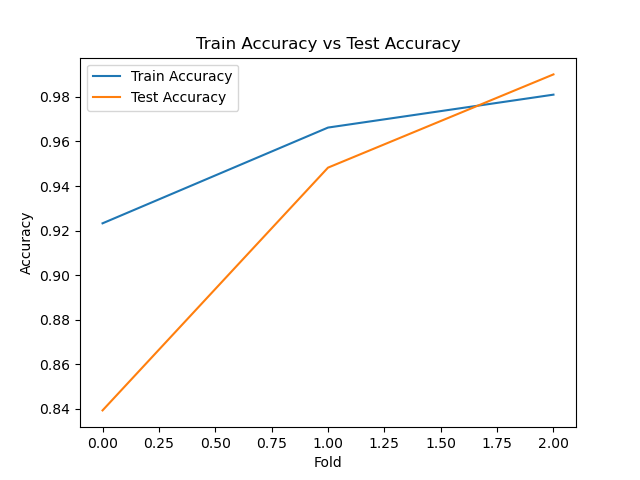
\includegraphics[width=\textwidth]{figures/cross_validation_100000_accuracy_3f.png}
        \end{subfigure}
        \begin{subfigure}{0.49\textwidth}
            \centering
            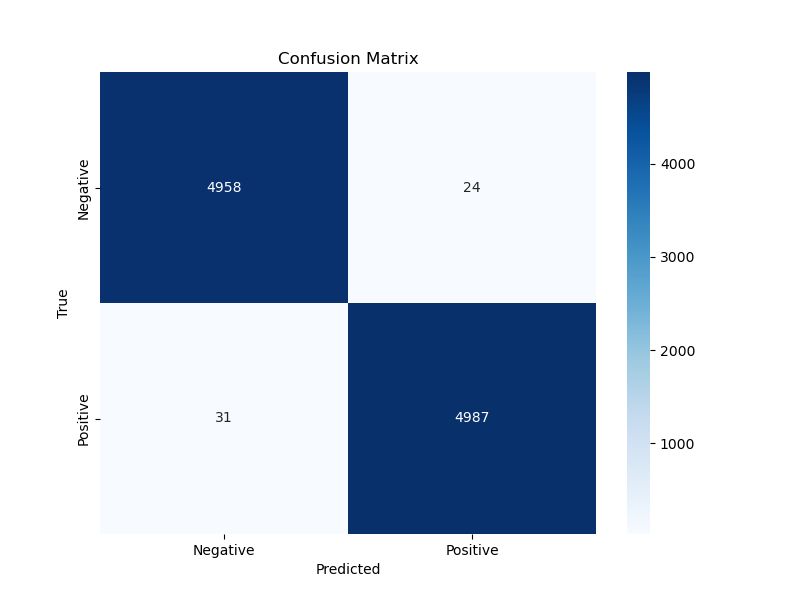
\includegraphics[width=\textwidth]{figures/cross_validation_100000_confusion_3f.png}
        \end{subfigure}
        \caption{Accuracy and confusion matrix for 3 fold cross-validation on 100,000 rows.}
    \end{figure}
    \FloatBarrier

    Finally, the model trained with 5 folds and 5,000 rows of data was tested on entirely unseen data, for this purpose 10 fake Reddit posts were created.

    \begin{python}
reddit_posts = ["Just landed my dream job! [SEP] I can't believe it finally happened. After months of interviews and applications, I got the job I've always wanted. Feeling on top of the world!",
"Had the best meal ever [SEP] Went to this new Italian restaurant downtown and it was amazing. The pasta was to die for and the service was impeccable.",
"Vacation was a blast! [SEP] Just got back from a week-long vacation in Hawaii. The beaches were stunning and the weather was perfect. Highly recommend!",
"Completed my first triathlon [SEP] After months of training, I finished my first triathlon. It was tough but so rewarding. Can't wait to do it again!",
"New hobby is so much fun [SEP] Started learning how to play the guitar and I'm loving it. It's challenging but incredibly satisfying when I nail a new song.",
"Worst customer service ever [SEP] Had a terrible experience at the electronics store. The staff were rude and completely unhelpful. Never going back.",
"Car problems again [SEP] My car broke down for the second time this month. It's so frustrating and costly to keep repairing it. Might have to buy a new one.",
"Disappointing movie night [SEP] Watched a highly anticipated movie and it was a total letdown. The plot was boring and the acting was subpar.",
"Feeling under the weather [SEP] Caught a nasty cold and have been feeling awful all week. Can't wait to get back to my usual self.",
"Bad dining experience [SEP] Went to a new sushi place and got food poisoning. Spent the night feeling miserable. Definitely won't be returning."]
    \end{python}

    When predicting the sentiment of these posts, the model predicted each one correctly, all with >99.9\% confidence, aside from one outlier with 97.13\% confidence.

    \FloatBarrier
    \begin{figure}[h]
        \centering
        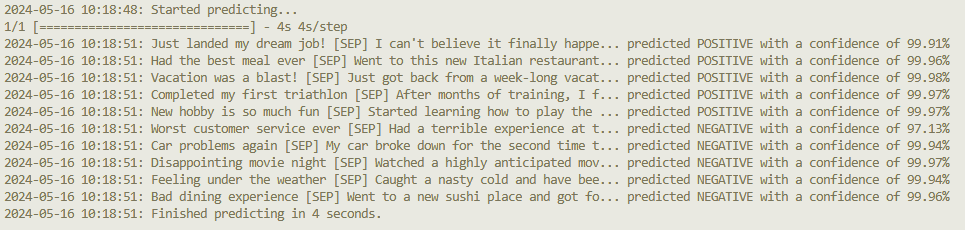
\includegraphics[width=0.95\textwidth]{figures/cross_validation_5000_predictions.png}
        \caption{Unseen predictions on 10 entries with 5 fold cross-validated model.}
    \end{figure}
    \FloatBarrier

    \subsection{Social Media Data Collection}
    To test the social media data collection, the functionality of \pinline{RedditScraper} must be assessed. This was accomplished by performing a simple unit test, to check that the program is capable of retrieving a post from a specified subreddit with specified search terms, along with its comments.
    \begin{python}
scraper = toolkit.RedditScraper()
posts, comments = scraper.search_sub('machinelearning', ['BERT', 'Transformers'], 1)
print(posts)
for comment in comments:
    print(comment)
    \end{python}

    \FloatBarrier
    \begin{figure}[h]
        \centering
        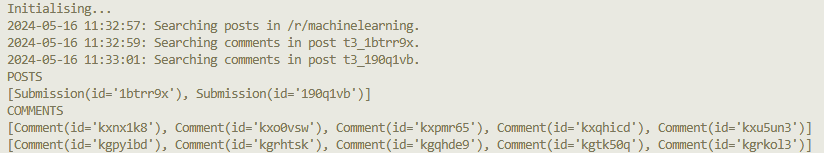
\includegraphics[width=0.95\textwidth]{figures/scrape-test.png}
        \caption{Results of testing social media data collection.}
    \end{figure}
    \FloatBarrier

    The content of these posts was also checked, to be sure that the given search terms were found and in the correct subreddit.

    \begin{python}
for post in posts:
    print(f"SUBREDDIT: {post.subreddit.display_name}")
    print(f"TITLE: {post.title}")
    print(f"BODY: {post.selftext}")
    \end{python}

    \FloatBarrier
    \begin{figure}[ht]
        \begin{minipage}[t]{0.45\textwidth}
            \centering
            \begin{tabular}{|p{7cm}|}
                \hline
                \textbf{/r/machinelearning} \\
                \hline
                \textbf{[D] SOTA BERT-like model?} \\
                \hline
                So we are all probably aware of state-of-the-art decoder only LLMs like GPT-4, Claude etc. These are great for generating text. But what I am not aware of is the SOTA BERT-like model. You know, things that can be used for tasks like NER, POS tagging, token classification. Are there models that are significantly better than say Roberta? \\
                \hline
            \end{tabular}
        \end{minipage}
        \hfill
        \begin{minipage}[t]{0.45\textwidth}
            \centering
            \begin{tabular}{|p{7cm}|}
                \hline
                \textbf{/r/machinelearning} \\
                \hline
                \textbf{[D] So, Mamba vs. Transformers... is the hype real?} \\
                \hline
                Heard all the buzz about Mamba, the new kid on the sequence modeling block. Supposedly it's faster, handles longer sequences better, and even outperforms Transformers on some tasks. But is it really a throne-stealer or just another flash in the pan? \\
                My perception: \\
                Strengths: Mamba boasts efficient memory usage, linear scaling with sequence length, and impressive performance in language and DNA modeling. Plus, it ditches the attention mechanism, potentially paving the way for faster inference. \\
                Weaknesses: Still early days, so Mamba's long-term stability and performance across diverse tasks remain to be seen. And while it doesn't need attention, its state space approach might be trickier to grasp for some folks. \\
                To the AI aficionados out there, is Mamba just the next shiny toy, or a genuine paradigm shift in sequence modeling? Will it dethrone the mighty Transformer, or coexist as a specialized tool? Let's hear your thoughts! \\
                \hline
            \end{tabular}
        \end{minipage}
        \caption{Posts with queries `BERT' and `Transformers' in /r/machinelearning.}
        \label{fig:reddit_posts}
    \end{figure}
    \FloatBarrier

    \subsection{Database management}
    The collected data is accurately and efficiently stored in \pinline{.json} format, one file for posts and one for comments, for each profile. The different profiles are also stored in \pinline{.json} format, storing information about the subreddits and queries to search.

    \FloatBarrier
    \begin{table}[ht]
        \centering
        \label{tab:bert_profile}
        \begin{tabular}{|l|l|}
            \hline
            \textbf{ID} & 3 \\
            \hline
            \textbf{Name} & BERT \\
            \hline
            \textbf{Subs} & \begin{tabular}[t]{@{}l@{}} `BERT', `Transformers' in /r/machinelearning \\
             `BERT', `Transformers' in /r/deeplearning \\
             `BERT', `Transformers' in /r/LanguageTechnology \end{tabular} \\
            \hline
        \end{tabular}
        \caption{Example brand profile}
    \end{table}
    \FloatBarrier

    \FloatBarrier
    \begin{figure}[ht]
        \begin{minipage}[t]{0.45\textwidth}
            \centering
            \begin{tabular}{|p{7cm}|}
                \hline
                \textbf{POST} \\  \hline \hline
                \textbf{ID:} 1btrr9x \\ \hline
                \textbf{Subreddit:} MachineLearning \\ \hline
                \textbf{Date/Time:} 1712039193 \\ \hline
                \textbf{Title:} [D] SOTA BERT-like model? \\ \hline
                \textbf{Body:} So we are all probably aware of state-of-the-art decoder only LLMs like GPT-4, Claude etc. These are great for generating text. But what I am not aware of is the SOTA BERT-like model. You know, things that can be used for tasks like NER, POS tagging, token classification. Are there models that are significantly better than say Roberta? \\ \hline
                \textbf{Score:} 72 \\ \hline
                \textbf{Comments:} ('kxnx1k8', 'kxo0vsw') \\ \hline
                \textbf{Sentiment:} Positive \\ \hline
            \end{tabular}
        \end{minipage}
        \hfill
        \begin{minipage}[t]{0.45\textwidth}
            \centering
            \begin{tabular}{|p{7cm}|}
                \hline
                \textbf{COMMENT} \\ \hline \hline
                \textbf{ID:} kxnx1k8 \\ \hline
                \textbf{PostID:} 1btrr9x \\ \hline
                \textbf{Subreddit:} MachineLearning \\ \hline
                \textbf{Date/Time:} 1712040433 \\ \hline
                \textbf{Body:} Deberta is still the goat \\ \hline
                \textbf{Score:} 65 \\ \hline
                \textbf{Sentiment:} Positive \\ \hline
            \end{tabular}
        \end{minipage}
        \caption{Retrieved first post and its first comment.}
        \label{fig:post_comment}
    \end{figure}
    \FloatBarrier

    \clearpage
    \subsection{Graphical User Interface}

        \subsubsection{Preliminary Usability Survey}
        This iteration of usability testing was conducted using the GUI wire-frames proposed during the design and methodology.

        \FloatBarrier
        \begin{table}[ht]
            \centering
            \caption{Preliminary Usability Survey Results}
            \label{tab:preliminary_usability_survey}
            \begin{tabular}{c|c}
                \textbf{Participant} & \textbf{Usability} \\
                \hline\hline
                Participant 1 & 7/10 \\ \hline
                Participant 2 & 6/10 \\ \hline
                Participant 3 & 8/10 \\ \hline
                Participant 4 & 7/10 \\ \hline
                Participant 5 & 6/10 \\
                \hline\hline
                \textbf{Average} & \textbf{6.8} \\
            \end{tabular}
        \end{table}
        \FloatBarrier
        As can be seen, this round of testing did not hit the desired usability score of 8/10, this meant that further refinement of the GUI was necessary before release.

        \subsubsection{Hands-On Usability Testing}
        Once the final, functional GUI was finalised, hands-on usability tests were conducted, for this purpose, the participants were supplied with a fully functional executable to use and rate, along with a short paragraph detailing their thoughts on the GUI.

        \FloatBarrier
        \begin{table}[ht]
            \centering
            \caption{Hands-On Usability Testing Results}
            \label{tab:hands_on_usability_testing}
            \begin{tabular}{c|c|p{8cm}}
                \textbf{Participant} & \textbf{Usability} & \textbf{Comments} \\
                \hline\hline
                Participant 1 & 7/10 & As someone who often struggles with technology, this is very easy to understand. I really enjoy the visual elements with charts and the simplicity to get results. [sec] \\ \hline
                Participant 2 & 9/10 & Everything is readable, make sense and seems functional. I got what I was supposed to do fast because every information is well laid out. My only complain would be that on the settings tab I would put the tabs to select the settings categories at the horizontal and not vertical which makes it easier to read and access what you want and also means you don't have to scroll to get to what you need (which a lot of basic users sometimes don't think about) [sec] \\ \hline
                Participant 3 & 9/10 & This was really well made and easy to use for the tech dummies, like me. Clear instructions and great functional programme. [sec] \\ \hline
                Participant 4 & 8/10 & It is very clear and usser friendly almost idiot proof. The graphs are clean and understandable. I will happily continue useing it for the forseeable future. [sec] \\ \hline
                Participant 5 & 10/10 & When first using the tool, I was able to create a profile and inputted some subreddits for analysis. the initial user interface was simple to understand and I managed to navigate around without any issues. I found the results easy to understand and found it very useful to be able to change between the sentiment graphs in order to further analyse the results. I would rate it a 10/10 due to its ease to navigate along with useful metrics being provided . [sec] \\
                \hline\hline
                \textbf{Average} & \textbf{8.6} & \\
            \end{tabular}
        \end{table}
        \FloatBarrier

        This round of testing managed to hit the required average usability score of 8/10, exceeding it by 0.6. This is a significant success for this project, showing that the GUI is intuitive and accessible to laypersons.

\section{Requirements Fulfillment}
This section aims to provide a link between the previously outlined requirements and assess whether they were fulfillment or not. There will also be a brief explanation on how the requirement was met or why it was not.

\begin{table}[h]
    \centering
    \caption{Non-Functional Requirements Checklist}
    \label{tab:non_functional_requirements}
    \begin{tabular}{p{6cm}|c|p{6cm}}
        \textbf{Requirement} & \textbf{?} & \textbf{Explanation} \\ \hline\hline
        \textbf{3.3.1} Optimize system performance for 10,000 posts/hr & HALF & Program has the capability, but Reddit API limits requests for the free version. \\ \hline
        \textbf{3.3.1} Average response time of 360 milliseconds & YES & Program is able to retrieve multiple posts in under a second. \\ \hline
        \textbf{3.3.2} Achieve minimum 8/10 usability score & YES &  \\ \hline
        \textbf{3.3.3} Develop a secure login system & NO & Lack of necessity due to anonymisation of data, as well as time constraints preventing it. \\ \hline
        \textbf{3.3.3} Utilise AES encryption for stored data & NO & Lack of necessity due to anonymisation of data, as well as time constraints preventing it. \\ \hline
        \textbf{3.3.4} Implement error handling and logging & HALF & While error handling was implemented, errors are only logged to the console, rather than in a window for the user. \\ \hline
        \textbf{3.3.4} Achieve 99.5\% application uptime & YES & Throughout testing, the GUI remained responsive outside of fringe cases during development. \\ \hline
        \textbf{3.3.5} Ensure accurate sentiment categorization >85\% & YES & Overcame expectations and achieved classification accuracies up to 99.9\% during testing. \\ 
    \end{tabular}
\end{table}

\begin{table}[h]
    \centering
    \caption{Functional Requirements Checklist}
    \label{tab:functional_requirements}
    \begin{tabular}{p{5cm}|c|p{6cm}}
        \textbf{Requirement} & \textbf{?} & \textbf{Explanation} \\ \hline\hline
        \textbf{3.2.1} Collect data from social media platforms & HALF & Successfully integrated the Reddit API. Due to new request limitations, X's API could not be integrated (\pinline{social.py}). \\ \hline
        \textbf{3.2.1} Accept .json files for brand reviews & NO & Possible disparities between inputted format and integrated format along with time constraints. \\ \hline
        \textbf{3.2.1} Anonymize personal data in collected data & YES & All mentions of both X and Reddit users are removed using regex substitution during text processing (\pinline{preprocess.py}). \\ \hline
        \textbf{3.2.1} Remove noise from text data & YES & URLs, subreddit mentions, and newlines removed. Stop-words remain, providing important context for BERT (\pinline{preprocess.py}). \\ \hline
        \textbf{3.2.1} Apply text normalization techniques & YES & Text normalisation techniques such as lemmatisation and stemming are implemented as options (\pinline{preprocess.py}). \\ \hline
        \textbf{3.2.2} Implement BERT for sentiment analysis & YES & BERT model has been implemented with training/fine-tuning, cross-validation, and predicting functionality (\pinline{model.py}). \\ \hline
        \textbf{3.2.2} Implement PFDualBERT for semantic relevance & NO & Although PFDualBERT proved to be powerful, due to time constraints it was not implemented. \\ \hline
        \textbf{3.2.2} Predict general sentiment around a term & YES & Sentiment prediction was used with specific subreddits and queries (\pinline{model.py}, \pinline{database.py}). \\ \hline
        \textbf{3.2.2} Predict sentiment polarity about specific aspects & NO & PFDualBERT was not implemented due to time constraints. \\ \hline
        \textbf{3.2.3} Analyze social-media data in real-time & HALF & Program has the capability, free Reddit API does not support so many requests (\pinline{social.py}, \pinline{database.py}, \pinline{analyse.py}). \\ \hline
        \textbf{3.2.3} Find new social-media posts with minimal delay & HALF & Program has the capability, Reddit API does not allow collecting posts from specific time-frame (\pinline{social.py}). \\ \hline
        \textbf{3.2.3} Save analyzed data for future recall & YES & Data saved in \pinline{.json} format (\pinline{database.py}). \\ \hline
        \textbf{3.2.4} Implement user-friendly interface & YES & GUI intuitively controls the underlying system (\pinline{interface.py}). \\ 
    \end{tabular}
\end{table}


\section{Reflection}
Through the implementation and testing of the sentiment analysis tool \citep{sentimentanalysistool}, many challenges were faced and overcome, while some proved too time-consuming to push through. The core components of the system, including sentiment analysis, social media interfacing, data management, and the GUI, underwent thorough evaluation against the predefined requirements.

The sentiment analysis model was based on the BERT architecture, fine-tuning the model to fit to the specific task of social media sentiment analysis. It exhibited promising accuracy during testing, however was found to be possibly over-fitting to the training data; due to this, other training methods were explored, such as cross-validation, which proved to be incredibly accurate and provided results exceeding expectations. However the promising PFDualBERT was unable to be implemented, as the complexity of the model was underestimated, as well as time constraints disallowing it.

Social media collection through was successfully implemented through the Reddit API, retrieving posts containing the correct queries in a timely manner. However, due to newly imposed API limitations, it was not possible to collect data in real-time, or collect large amounts of data at a time. Specifically, the X API was entirely unusable for the purpose of collecting post data, and so it was necessary to make the application more Reddit-centric, which actually made the program architecture simpler to implement, and resulted in a more sensible implementation.

The database management implementation proved to be efficient and scalable, with JSON providing a simple format and facilitating efficient reading and writing of data. However, it was not possible to implement AES encryption or a login system due to time constraints.

The GUI took up a large chunk of the development time, and was the main cause of time constraints for other parts of the program. However, after the initial design proposal and feedback, the GUI showed a high usability score, making the extra time spend worthwhile.

Overall, the development process went incredibly smoothly, and produced very satisfiable results, with meaningful considerations for future development.

\section{Future Considerations}
To address the unmet requirements and expand the functionality of the application, future work should focus on refining the planning process, leveraging and testing more pre-trained models, and exploring sentiment polarity prediction with PFDualBERT and other ABSA models. For this to be a market-ready solution, the application should implement proper security measures, allowing the use of the user's own API credentials, and integrate more advanced, customisable analytical tools. On top of this, incorporating user feedback is necessary to the improvement of this tool.


\chapter{Conclusion}
In conclusion, the development and evaluation of the sentiment analysis tool has provided significant insight into harnessing natural language processing techniques for social media sentiment analysis. Through leveraging deep-learning models like BERT, the tool has demonstrated great success in the sentiment classification of social media posts.

Throughout the project, several critical insights were gained regarding model training, data management, and graphical user interface design. Various challenges such as over-fitting, resource constraints, API limitations, and time constraints were addressed, proving great adaptability and problem-solving skills.

Despite the success achieved in multiple areas, it is important to acknowledge the improvements that must be made to ensure an application suitable for public release. Time constraints were the main culprit for preventing the implementation of certain features, highlighting the need for better planning and a more robust development process.

Looking ahead, the project has several avenues for further exploration. Future versions of the tool could benefit by integrating additional pre-trained models, expanding support into different social medias or review sites, or implementing additional analytics features. These improvements should be paired with a robust development process to ensure the achievability of each feature.

Overall, this project has been a great learning experience, allowing the exploration of natural language processing and sentiment analysis, as well as deep-learning models such as BERT. It has laid the foundation for continued research and development within this area of computer science.

\printReferences

\end{document}
